%%%%%%%%%%%%%%%%%%%%%%%%%%%%%%%%%%%%%%%%%%%%%%%%%%%%%%%%%%%%%%%%%%%%%%%%
%Desarrollo de un juego para Nintendo DS | Trabajo de Fin de Grado
% Escuela Politécnica Superior de la Universidad de Alicante
% Realizado por: Carla Maciá Díez
% Contacto: carlamd1997@hotmail.com / cmd23@alu.ua.es
%%%%%%%%%%%%%%%%%%%%%%%%%%%%%%%%%%%%%%%%%%%%%%%%%%%%%%%%%%%%%%%%%%%%%%%%

\chapter{Desarrollo} 

En este capítulo se describirá detalladamente el proceso realizado para conseguir el juego que se ha diseñado previamente. Se explicará desde todas las herramientas que se necesitan hasta el producto final, pasando por unas primeras demos básicas de manejo de la consola y su hardware, mínimo producto viable e iteraciones y problemas del mismo, de esta manera conseguimos que cualquier persona que busque información sobre desarrollo en NDS le sea lo más útil posible y sea capaz de buscar las partes que más le interesan.

\section{Herramientas}

\subsection{Entorno de desarrollo}

El lenguaje de programación que vamos a utilizar es \textbf{C++} debido a varios motivos, entre ellos que la librería es para dicho lenguaje y además es el perfecto candidato para dejarnos aprovechar la máquina en su totalidad.

\vspace{0.5cm}

Por último, para programar necesitaremos un editor de texto. En mi caso he utilizado \textbf{Sublime Text 3} por comodidad, pero cualquiera es completamente válido.

\subsection{Emuladores}

Para probar el juego que vamos a desarrollar es indispensable disponer de programas que \textbf{emulen virtualmente la consola} en nuestro ordenador de trabajo. Esto no solo nos \textbf{ahorra el tiempo} que cuesta en probarlo en una máquina real, también nos proporciona un \textbf{entorno seguro} donde no importa si metemos demasiado la pata haciendo nuestras pruebas, ya que no hay riesgo alguno de romper una máquina real.

\vspace{0.5cm}

Existen gran cantidad de emuladores de Nintendo DS, pero nos vamos a centrar en dos de ellos.

\vspace{0.5cm}

El primero de ellos es \textbf{Desmume}. Este es bastante \textbf{cómodo} ya que se encuentra disponible tanto para Windows, Mac y Linux, y también nos permite cambiar los controles y unos pequeños ajustes que nos pueden servir para depurar nuestros programas. Es una muy buena opción si lo que queremos es probar nuestros programas de una manera \textbf{rápida} o incluso ejecutar los ejemplos que nos proporciona la librería, de la cual hablaremos más adelante.

\clearpage

\begin{figure}[htbp]
\centering
  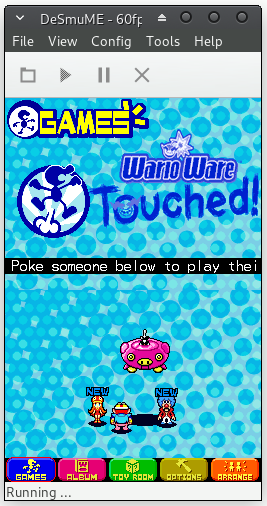
\includegraphics[width=0.3\textwidth]{archivos/desmume.png}
  \caption{Desmume emulando WarioWare: Touched!}
  \label{fig:desmume}
\end{figure}

\vspace{0.5cm}

Por otro lado tenemos \textbf{no\$gba}, una excelente opción y sin duda la que más vamos a \textbf{necesitar} usar. Permite ejecutar tanto ROMs de GBA como de NDS y además tiene disponible una \textbf{versión \textit{debug}} con muchísimas más opciones que Desmume. Entre ellas un visualizador de toda la memoria de la consola así como herramientas de \textbf{depurado visual} para \textbf{fondos, sprites y paletas}.

\clearpage
\begin{figure}[htbp]
\centering
  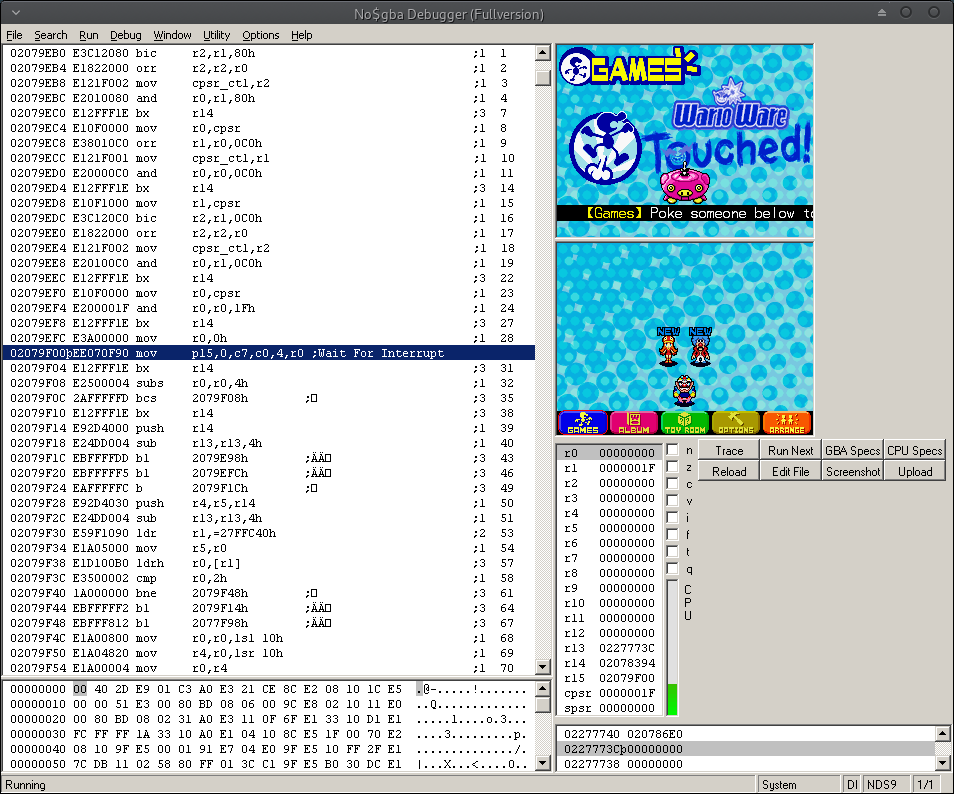
\includegraphics[width=0.5\textwidth]{archivos/nogba.png}
  \caption{Versión debug de no\$gba emulando WarioWare: Touched!}
  \label{fig:nogba}
\end{figure}

\begin{figure}[htbp]
\centering
  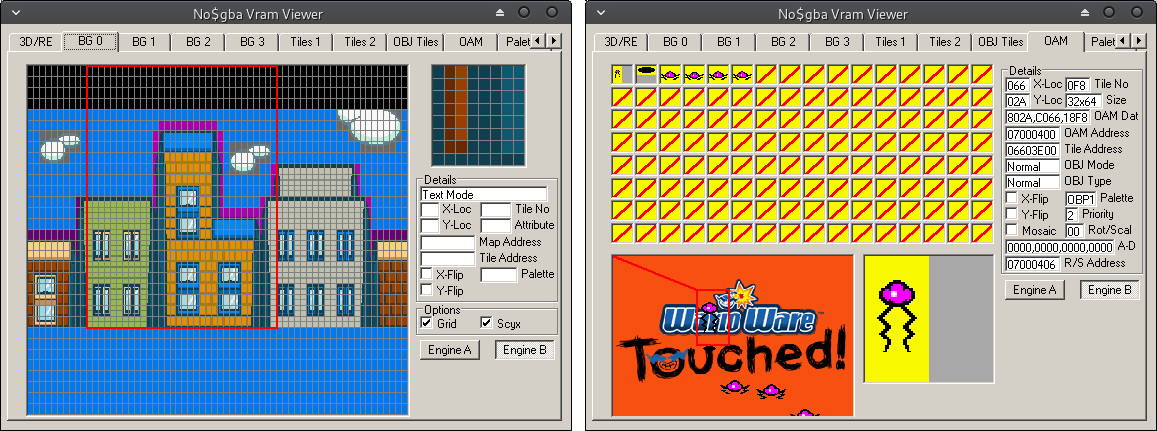
\includegraphics[width=0.7\textwidth]{archivos/nogba1.png}
  \caption{Herramienta de depurado para fondos (izquierda) y sprites (derecha) de no\$gba}
  \label{fig:nogba1}
\end{figure}

\vspace{0.5cm}

Como única pega es que \textbf{solo} está \textbf{disponible} para el sistema operativo \textbf{Windows}, pero sin mucho problema podemos hacer que funcione en Linux gracias al uso de la herramienta \textbf{Wine}.

\vspace{0.5cm}

%Para conocer más acerca de cómo descargar y probar estos emuladores continúa en el Anexo...

\vspace{1cm}

\subsection{Cartuchos Flash}

Aunque dispongamos de los emuladores para la gran mayoría del trabajo, es imprescindible probar los resultados de vez en cuando en una \textbf{máquina real}. Para ello evidentemente deberemos disponer de la consola en sí, pero también necesitaremos un \textbf{cartucho} al cual introduciremos \textbf{nuestro programa} y éste será ejecutado por la consola. Estos son los \textbf{cartuchos flash}. 

\vspace{0.5cm}

Se denominan de esa forma ya que poseen una memoria flash, que permite \textbf{simultáneas lecturas y escrituras} en una misma operación. Esta tecnología se emplea en las unidades de \textbf{almacenamiento externos} (USB) o \textbf{discos sólidos} (SSD)

A continuación vamos a centrarnos en una marca de cartucho flash concreta, ya que es la que poseemos para desarrollar el proyecto.

\subsubsection{R4}

\textbf{Revolution for NDS} o \textbf{R4 DS} nació principalmente para la \textbf{piratería} de juegos de NDS o para ejecutar aplicaciones ilegales en ella. Se trata de un cartucho similar a los originales de los juegos de NDS con una \textbf{ranura} para una tarjeta \textbf{MicroSD}, a la cual nosotros copiaríamos nuestro fichero binario con extensión nds y eso bastaría para probar el juego. Posee también una \textbf{interfaz agradable}, permitiendo también la \textbf{reproducción de contenidos multimedia} en una sección de esta.

\vspace{0.5cm}

\begin{figure}[htbp]
\centering
  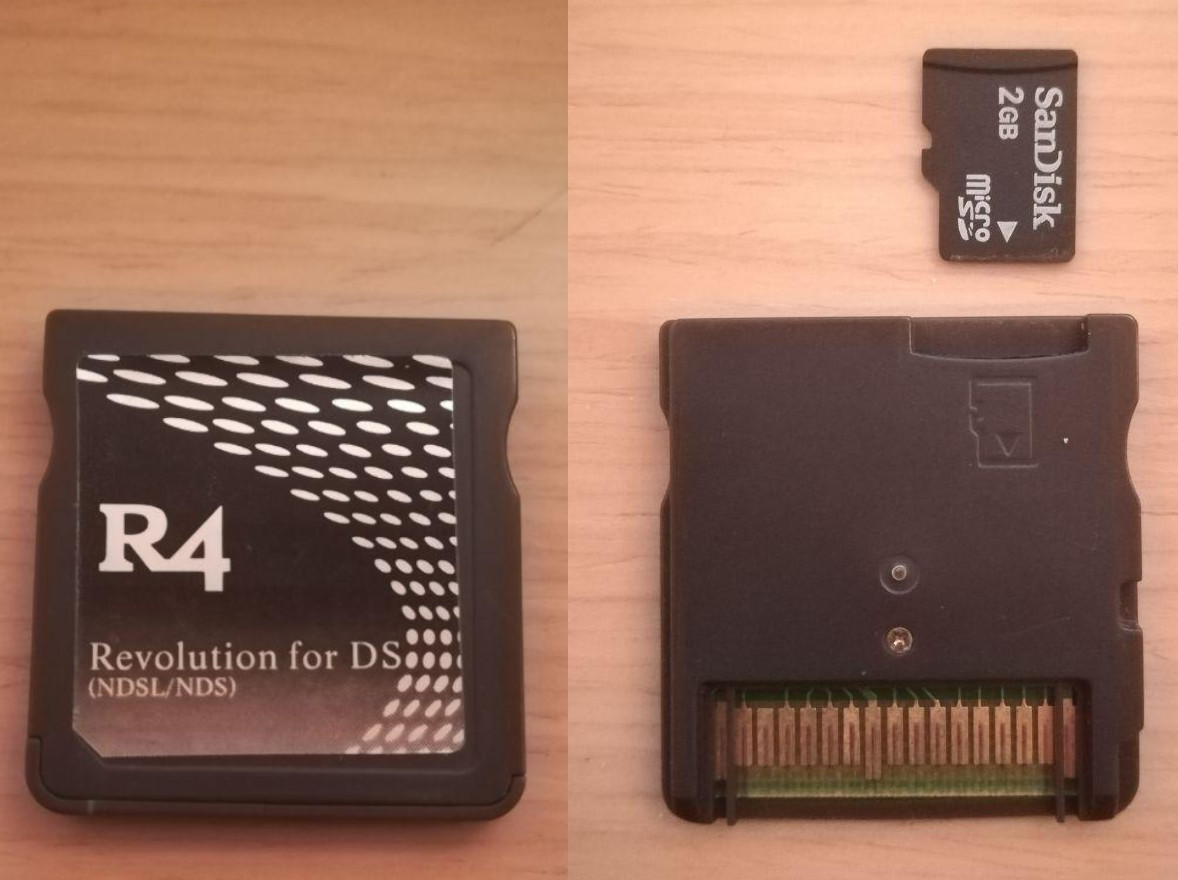
\includegraphics[width=0.6\textwidth]{archivos/r4.jpg}
  \caption{Cartucho R4}
  \label{fig:r4}
\end{figure}

\vspace{1cm}

\subsection{DevkitPro}

\textbf{DevkitPro} es una \textbf{colección} de gran cantidad de \textbf{herramientas} de ayuda para \textbf{desarrollar} en sistemas como NDS, GBA, GameCube, Wii, Nintento Switch... Digamos que es como Adobe. Nosotros no usamos Adobe para editar imágenes digitales, en su lugar usamos Photoshop, desarrollado por este. En nuestro caso, nosotros usaremos una herramienta de devkitPro para poder \textbf{compilar} nuestro programa y \textbf{generar los binarios} adecuados para ejecutarlos en los procesadores ARM de la consola, esta herramienta es \textbf{devkitARM}.

\vspace{0.5cm}

%Para saber cómo instalar y conocer más a fondo devkitARM continuar en el Anexo...

\subsection{Libnds}

La librería que utilizaremos es\textbf{ libnds}. Inicialmente fue desarrollada por Michael Noland (alias joat) y Jason Rogers (alias rovoto), pero después de unos meses pasó a manos de Dave Murphy (alias WinterMute), quien a día de hoy es la principal persona que la mantiene.

\vspace{0.5cm}

Libnds empezó siendo un simple \textbf{conjunto de macros y definiciones} de zonas de memoria de \textbf{recurrente acceso} para \textbf{facilitar} el uso y legibilidad del código a los \textbf{programadores}. Por ejemplo, es lo mismo escribir SPRITE\_GFX que 0x6400000, ambas hacen referencia al lugar en memoria donde comienza el almacenamiento de datos referente a los sprites, pero la primera es sin duda \textbf{más limpia y fácil de entender}, y sobre todo le quita peso al programador ya que no le obliga a conocerse todas estas posiciones con exactitud.

\vspace{0.5cm}

Más tarde y según los desarrolladores homebrew comenzaban a usar libnds, se le empezaron a \textbf{añadir elementos} de gran utilidad, como por ejemplo \textbf{estructuras de datos} o incluso \textbf{APIs para crear sprites} y alocarlos en memoria, simplificando el trabajo del programador a simplemente llamar a un par de \textbf{funciones}. A día de hoy cubre gran cantidad de aspectos como gráficos, sonido, pulsaciones de botones y pantalla táctil, operaciones matemáticas complejas... y es usada por el 90\%  de la comunidad.

\vspace{1cm}

\subsection{Grit}

\textbf{GBA Raster Image Transmogrifier} o Grit para los amigos, es una herramienta de \textbf{conversión de mapas de bits para el desarrollo en GBA y NDS}. Es decir, es una herramienta que nos aydará a \textbf{convertir nuestras imágenes} de fondos, sprites o tiles en algo que la \textbf{máquina} pueda \textbf{entender}.

\vspace{0.5cm}

Acepta muchos tipos de \textbf{formatos} de imágenes como BMP, PNG, GIF, JPG... y también nos permite \textbf{trabajar con ellas} para cambiar la profundidad de bit, separar nuestros fondos en tiles de manera rápida, soporte para transparencias y mucho más. 

\vspace{0.5cm}

Lo que más nos va a interesar a parte de que nos convierta las imágenes en binarios que la NDS entienda, es que además nos proporciona un \textbf{archivo de cabecera} con definiciones que podemos \textbf{usar en nuestro programa} como el tamaño de la imágen en bytes, anchura y altura y e información relativa a su paleta. Esto ya lo veremos más adelante en el desarrollo, pero ya adelanto que es una herramienta muy útil y nos va a ahorrar muchos problemas.

\vspace{0.5cm}

 Aunque grit compila en todas las plataformas, para sistemas que no se traten de Windows debemos \textbf{crearnos nuestro propio makefile}. Esto no será mucho problema, pues en los \textbf{ejemplos de libnds} ya vienen makefiles que incluyen el uso de esta herramienta. En \textbf{Windows} disponemos de la versión \textbf{Wingrit} con una interfaz que nos permitirá trabajar con la imágen de manera más sencilla y visual. Para el resto de sistemas operativos tenemos la \textbf{versión por comandos}, que es la que utilizaremos nosotros la mayor parte del tiempo. Una vez instalado grit en nuestro sistema (Linux Manjaro en este caso), podemos abrir una terminal y ejecutar el comando "grit" para leer una pequeña \textbf{descripción de todos los comandos} que se encuentran disponibles.
 
 \begin{figure}[htbp]
\centering
  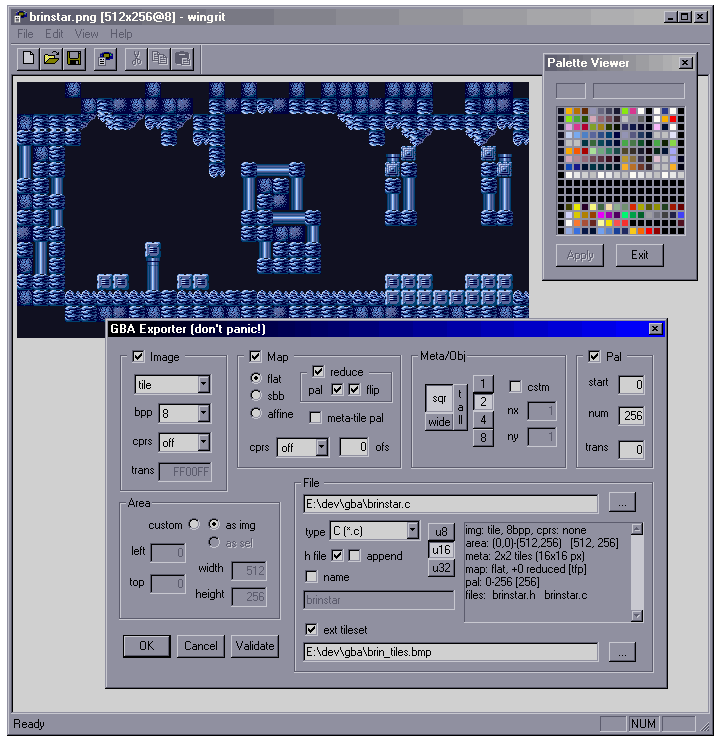
\includegraphics[width=0.5\textwidth]{archivos/wingrit.png}
  \caption{Wingrit, versión GUI para Windows de Grit}
\textbf{Fuente:} \href{https://www.coranac.com/man/grit/html/wingrit.htm}{Coranac}
  \label{fig:wingrit}
\end{figure}

\clearpage

\begin{figure}[htbp]
\centering
  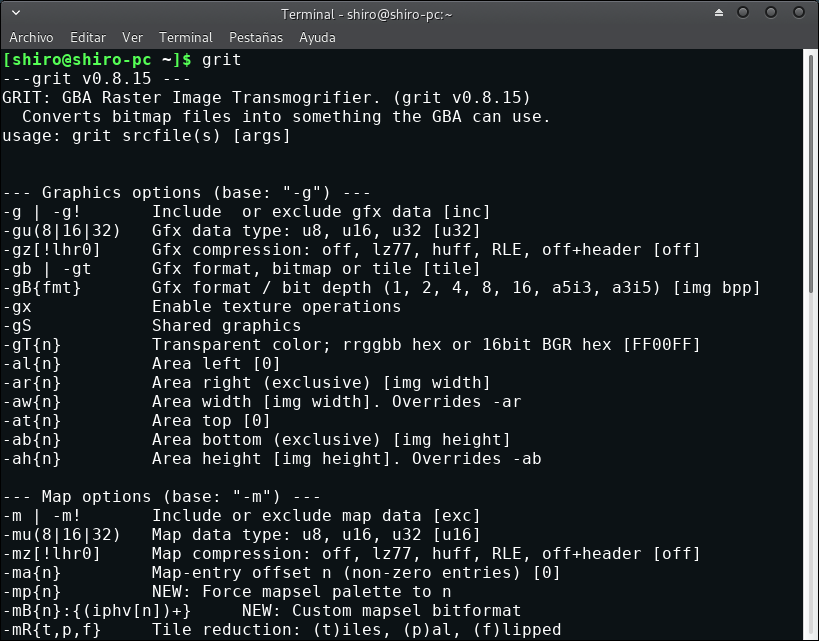
\includegraphics[width=0.6\textwidth]{archivos/gritcomand.png}
  \caption{Grit versión comandos}
  \label{fig:grit}
\end{figure}

 
 \vspace{0.5cm}

 Además, se trata de un proyecto \textit{open-source}, por lo que si poseemos del conocimiento  adecuado podemos añadir nuestro propio código para personalizar el uso.

 \vspace{1cm}

\section{Iteraciones}

\subsection{Iteración 0 - Investigación previa y primeros pasos en NDS}

Esta primera iteración se dedicó a documentarse sobre el desarrollo en NDS, la consola y su hardware, así como conocer todas las herramientas necesarias para comenzar a trabajar en el proyecto. También se realizaron una serie de pruebas para aprender cómo pintar gráficos en pantalla. A esta iteración se le dedicó especialmente más tiempo ya que era la que quería conocer con mayor detalle, pues luego se quería plasmar bien en esta memoria esos pasos de modo que se pudiese entender de la forma más clara posible.

\subsubsection{Fondos}
\vspace{0.5cm}

Una vez ya tenemos todas las herramientas necesarias podemos ponernos manos a la obra a programar. Sin embargo, antes de ponernos a programar nuestros juegos vamos a realizar una serie de pruebas y así ir conociendo el hardware de la NDS. En concreto, en esta sección vamos a aprender a \textbf{dibujar fondos en ambas pantallas}.

\vspace{0.5cm}

Primero que todo vamos a crear la carpeta del proyecto. Esta carpeta se llamará "Fondos", y dentro contendrá una serie de carpetas dedicadas a distintos ficheros. En una carpeta "gfx" almacenaremos todas las imágenes del juego. En una carpeta "include", introduciremos los archivos de cabecera y, en una carpeta "source" todos los archivos .cpp del proyecto. Esto lo haremos así ya que vamos a usar el Makefile que viene en los ejemplos de devkitPro para compilar nuestro proyecto y que nos genere un archivo ejecutable. Este sería el aspecto de la carpeta:

\vspace{0.5cm}

\begin{figure}[htbp]
\centering
  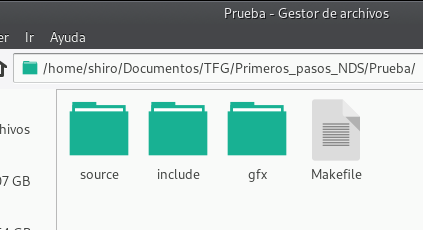
\includegraphics[width=0.6\textwidth]{archivos/carpetas.png}
  \caption{Carpeta del proyecto}
  \label{fig:carpetas}
\end{figure}

\vspace{0.5cm}

Una vez lo tenemos, creamos el archivo main.cpp, que contendrá el bucle principal del juego. Necesitamos mantener la consola este ya que de otro modo nuestro programa llegará a su fin, la consola se reiniciará y no nos dará tiempo a ver los resultados de nuestras pruebas. Nuestro main contendrá el siguiente código código:

\begin{lstlisting}[caption={Bucle principal del juego}, label={code:gameloop}]

#include <nds.h>

int main(void){
    while(1){ //bucle infinito
        //actualizamos el juego
    }
}
\end{lstlisting}

\vspace{0.5cm}

Como se puede ver en el \hyperref[anexo]{\textbf{Anexo I}}., el hardware de esta consola posee \textbf{dos motores gráficos}, uno para \textbf{cada pantalla}. Por lo general, libnds asigna el primer motor (al que llamaremos \textbf{motor A}) a la \textbf{pantalla superior} y el segundo (\textbf{motor B}) a la \textbf{pantalla táctil}, pero nosotros podemos cambiarlo si así lo deseamos.

\vspace{0.5cm}

De entre  todos los modos en los que puede operar cada motor, el que más nos interesa es el \textbf{modo 5}. Este modo permite que dos de los cuatro fondos disponibles en cada pantalla sean del tipo \textit{"Extended Rotation Background''}. Esto quiere decir que tienen la capacidad de ser \textbf{rotados, escalados o trasladados} mediante una \textbf{matriz afín} de transformaciones, que veremos más adelante. 

\vspace{0.5cm}

Vamos a comenzar preparando ambos motores para usarlos, para ello libnds nos lo pone muy simple ofreciendonos la función powerOn(), que "enciende'' un hardware específico. En este caso bastaría con símplemente enviarle como parámetro POWER\_ALL\_2D.

\vspace{0.5cm}

Después debemos realizar el mapeo de la memoria de video para que la consola sepa en qué zonas debe copiar los datos de los fondos. Como ya se ha comentado anteriormente, la NDS posee 9 bancos de VRAM, en este caso vamos a mapear el banco A como almacenamiento de fondos para la pantalla superior y el banco C para la inferior, pero podemos asignarlos a nuestro gusto. Para ello, usaremos las funciones vramSetBank de libnds.

\vspace{0.5cm}

\begin{lstlisting}[caption={Mapeo de memoria de video}, label={code:setbanks}]
vramSetBankA(VRAM_A_MAIN_BG_0x06000000);
vramSetBankC(VRAM_C_SUB_BG_0x06000000);
\end{lstlisting}

\vspace{0.5cm}

Una vez hecho esto debemos establecer a ambos motores el modo de vídeo deseado, así como especificarles las capas de fondos que van a estar activas. Esto lo haremos con las funciones videoSetMode y videoSetModeSub.

\vspace{0.5cm}

\begin{lstlisting}[caption={Bucle principal del juego}, label={code:gameloop}]
videoSetMode(MODE_5_2D | DISPLAY_BG3_ACTIVE);
videoSetModeSub(MODE_5_2D | DISPLAY_BG3_ACTIVE);
\end{lstlisting}

\vspace{0.5cm}

Casi hemos terminado preparando los fondos para dibujar, pero aún debemos dar valor a una serie de regístros de control específicos de cada fondo para indicarle qué datos le vamos a copiar, dónde y cómo los posiciona en pantalla.

\vspace{0.5cm}

\begin{lstlisting}[caption={Bucle principal del juego}, label={code:gameloop}]
REG_BG3CNT = BG_BMP16_256x256 | BG_BMP_BASE(0) | BG_PRIORITY(3);
\end{lstlisting}

\vspace{0.5cm}

En concreto, en esta última línea le hemos porporcionado la siguiente información:

\vspace{0.5cm}

\begin{itemize}
 \item \textbf{BG\_BMP16\_256x256: } El fondo sera un bitmap de 16 bits de profundidad y de 256 píxeles de ancho y alto como máximo.
  \item \textbf{BG\_BMP\_BASE(0):} Lugar en memoria donde se localizará el fondo.
   \item \textbf{BG\_PRIORITY(3)}: Le asigna el nivel 3 de prioridad. La prioridad en los fondos va de 0 (encima) a 3 (debajo) y se usa para decidir qué fondos se visualizan por encima de los demás.

\end{itemize}

\vspace{0.5cm}

Ahora volvemos al tema que habíamos dejado antes, la matriz afín. Los registros que vienen a continuación sirven para modificar esa matriz y aplicar así transformaciones a los fondos. Como de momento no queremos aplicarle transformación alguna, lo ideal es que la dejemos como una matriz identidad.

\vspace{0.5cm}

\begin{figure}[htbp]
\centering
  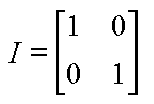
\includegraphics[width=0.2\textwidth]{archivos/matrizid.png}
  \caption{Matriz identidad}
  \label{fig:idmatr}
\end{figure}

\vspace{0.5cm}

\begin{lstlisting}[caption={Registros de control para la matriz afín de los fondos}, label={code:gameloop}]
REG_BG3_PA = 1 << 8;
REG_BG3_PB = 0;
REG_BG3_PC = 0;
REG_BG3_PD = 1 << 8;
\end{lstlisting}

\vspace{0.5cm}

Como podemos ver, en los registros donde van los unos a continuación aparece ``<<``. Este es el operador desplazamiento, sirve para desplazar los bits en el sentido al que apuntan tanto como indique el valor de la derecha. En ese caso, el 0000000000000001 (en binario) que asignabamos a los registros pasa a ser 0000000100000000. Pero, ¿para qué queremos eso?

\vspace{0.5cm}

Esto tiene que ver con cómo interpreta la NDS los bits. En el sistema binario hay varias formas de representar un número, como la coma fija. Esta nos permite representar números fraccionarios, lo cual nos interesa al para poder expresar senos o cosenos que nos servirán para rotar la imágen.

\vspace{0.5cm}

\begin{figure}[htbp]
\centering
  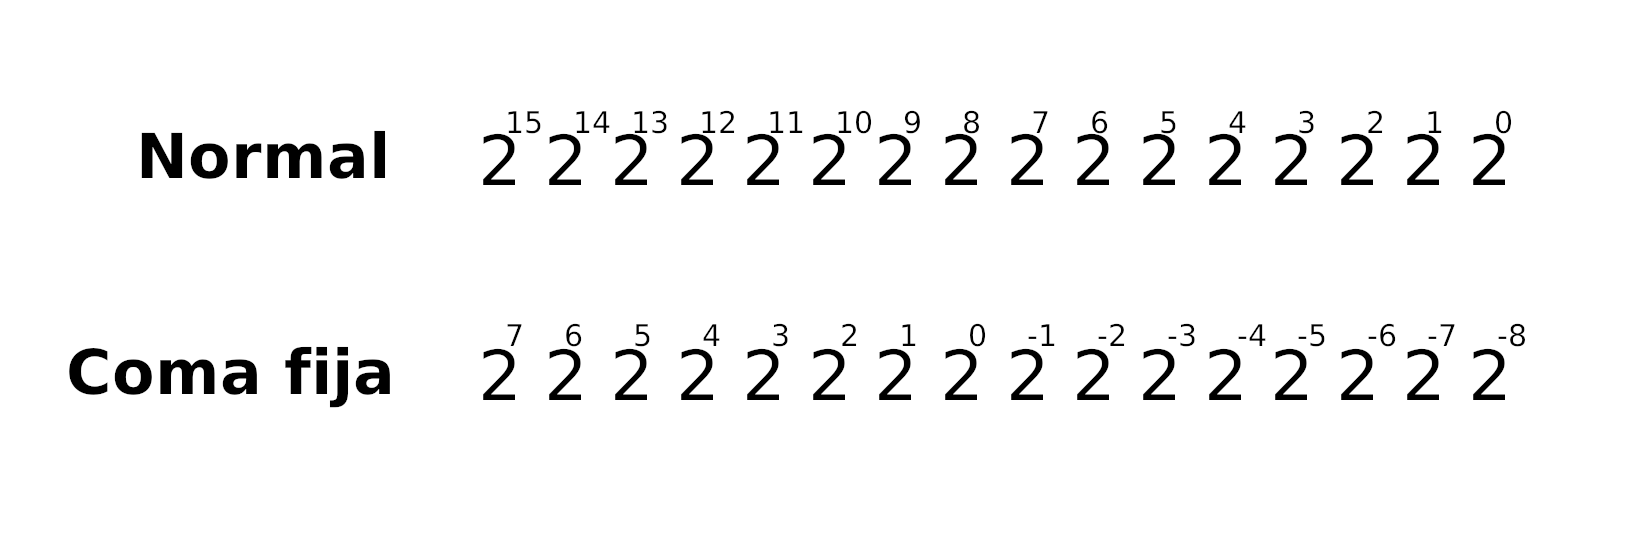
\includegraphics[width=0.7\textwidth]{archivos/comafija.png}
  \caption{Diferencias entre la representación normal binaria y la coma fija}
  \label{fig:}
\end{figure}

\vspace{0.5cm}

Lo último que faltaría para ver nuestros fondos en la consola sería copiar los bytes de las imágenes a la zona de memoria que corresponde. Aquí es donde entra Grit para facilitarnos el trabajo. En la carpeta gfx copiaremos nuestra imágen, así como también incluiremos un archivo con extensión .grit que contendrá lo siguiente:

\vspace{0.5cm}

\begin{lstlisting}[caption={Comandos de grit por archivo}, label={code:gritarchive}]
#Nombre del símbolo. Indica el nombre dentro de nuestro programa
-s ground

# Warning/log level. [1-3] Muestra todos los mensajes de error o warnings. Nos interesa tenerlos activados para depurar.
-W3

# Indica si el fondo tiene transparencia. Si no tiene -> !.  Si tiene indicar el valor en hexadecimal del color transparente.
-gT!

# Bitmap image. Indica si es un mapa de bits o tiles, en este caso de bits
-gb

# Bit depth. Indica la profundidad de bit
-gB16
\end{lstlisting}

\vspace{0.5cm}

Así pues, al compilar grit realizará la conversión de todas las imágenes que se encuentren en la carpeta gfx de nuestro proyecto. Esta conversión se hará utilizando las reglas que se establecen el el archivo anterior, pero si no existe uno se aplicarán las de por defecto. Por último creará una cabecera con datos de nuestra imágen.

\vspace{0.5cm}

Con esto ya solo nos faltaría copiar los bytes de la imágen a la memoria de video de la consola. Esto lo haremos usando la función de C++ memcpy.

\vspace{0.5cm}

\begin{lstlisting}[caption={Copia de la imágen en la memoria de video}, label={code:vramcopy}]
memcpy((uint16*)BG_BMP_RAM(0), groundBitmap, groundBitmapLen);
                                //destino                               //origen                    //tamanyo a copiar                                  
\end{lstlisting}

\vspace{0.5cm}

BG\_BMP\_RAM(BASE) es una macro que dado un valor en  BASE calcula una dirección de memoria. Por ejemplo, para BASE igual a 2, calculará 2 * 4000 y el resultado se lo sumará a 6000000 (todas las operaciones en base 16, es decir, hexadecimal). Como nosotros queremos copiar nuestro fondo en 0x06000000 como valor a BASE tenemos que pasarle un 0. Sin embargo, si en lugar del banco A hubíesemos elegido el banco B (0x06020000) debería valer 8 (8 * 4000 + 6000000 = 0x06020000).

\vspace{0.5cm}

Ya podemos compilar nuestro programa y, si todo ha salido bien deberíamos tener un resultado como el siguiente:

\vspace{0.5cm}

\begin{figure}[htbp]
\centering
  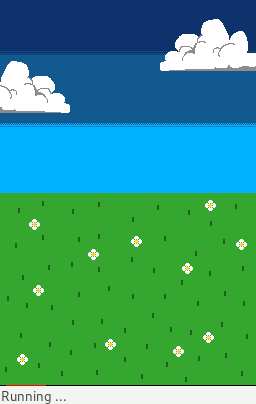
\includegraphics[width=0.4\textwidth]{archivos/fondos.png}
  \caption{Resultado en el emulador Desmume}
  \label{fig:fondo}
\end{figure}

\vspace{0.5cm}

\subsubsection{Sprites}

A la hora de dibujar sprites debemos realizar una serie de tareas adcionales, pues vamos a trabajar con la OAM.

\vspace{0.5cm}

Lo primero es, como anteriormente, mapear un banco de memoria de vídeo a memoria para sprites. Esto se puede hacer con la funcion vramSetBankE() y la macro VRAM\_E\_MAIN\_SPRITE. Además, debemos especificar también en el modo de vídeo que se visualicen los sprites y que su forma de guardarlos en memoria va a ser lineal (DISPLAY\_SPR\_1D).

\vspace{0.5cm}

\begin{lstlisting}[caption={Mapeo del banco E a memoria de sprites}, label={code:vrame}]
	vramSetBankE(VRAM_E_MAIN_SPRITE);
	[...]
	videoSetMode(MODE_5_2D |  DISPLAY_SPR_ACTIVE | DISPLAY_SPR_1D);
\end{lstlisting}

\vspace{0.5cm}

Una vez hecho esto, debemos copiar la información del sprite a memoria, tal y como hacíamos con los fondos, con el añadido de que ahora sí necesitamos copiar también la paleta. Grit también nos proporciona la paleta del sprite, siempre que le pasemos el parámetro -p. En el archivo de cabecera del sprite tenemos las variables spritePalLen como el tamaño que ocupa la paleta y spritePal, un puntero a dónde comienza esta.

\vspace{0.5cm}

\begin{lstlisting}[caption={Copia de la información de sprites a memoria de video}, label={code:spritememcpy}]
memcpy(&SPRITE_GFX[0], spriteTiles, spriteTilesLen);
memcpy(&SPRITE_PALETTE[0], spritePal, eyes_1PalLen);
\end{lstlisting}

\vspace{0.5cm}

Una vez hemos hecho esto, ya podemos trabajar con la OAM para crear nuestros sprites.

\vspace{0.5cm}

La OAM está formada objetos de tipo SpriteEntry y SpriteRotation. El primero de ellos guarda información relativa al sprite en sí, como su posición en pantalla, tamaño en pixeles, modo de color, etc. Por otro lado, el segundo de ellos guarda información relativa a las transformaciones afines que se aplican a ese sprite en concreto, tal y como hacíamos con los fondos.

\vspace{0.5cm}

Ahora bien, durante la ejecución normal de un juego, lo típico es que tengamos varios sprites, y en un mismo ciclo cambiemos algo de casi todos ellos, por ejemplo si tenemos muchos enemigos a cada uno le tendremos que cambiar su posición o lo tendremos que animar. Es por ello que trabajar diréctamente sobre la OAM puede no ser la mejor idea, pues acceder a memoria supone un coste elevado. En su lugar, podemos crearnos una copia de la OAM que nosotros guardaremos en caché y, una vez por ciclo, volcar toda esa copia en la memoria real. Pero es muy importante que no pasemos por alto inicializar dicha copia.

\vspace{0.5cm}

Esto podemos llevarlo a cabo gracias a la estructura OAMTable de libnds, que contiene tanto los objetos de tipo SpriteEntry como SpriteRotation.

\vspace{0.5cm}


\begin{lstlisting}[caption={Declaración de la copia de la OAM y}, label={oamupdate}]
OAMTable* oam; //Nuestra copia de la OAM

[...]

//Inicializamos la copia de la OAM poniendo todos sus atributos a 0
void Graphics::initOAM(){

   	SpriteEntry* se;
	SpriteRotation* sr;

	for(int i = 0; i < SPRITE_COUNT; i++){
		se = &oam->oamBuffer[i];
		se->attribute[0] = ATTR0_DISABLED;
		se->attribute[1] = 0;
		se->attribute[2] = 0;
	}

	for(int j = 0; j < MATRIX_COUNT; j++){
		sr = &oam->matrixBuffer[j];
		sr->hdx = 1 << 8;
		sr->hdy = 0;
		sr->vdx = 0;
		sr->vdy = 1 << 8;
	}
}


[...]

//volcamos la copia de la OAM en la OAM real
void Graphics::updateOAM(){
	memcpy(OAM,oam->oamBuffer,SPRITE_COUNT * sizeof (SpriteEntry));
}

\end{lstlisting}

\vspace{0.5cm}

Por último, solo quedaría crear un sprite y ver si se dibuja en pantalla. Esto lo haremos creando un objeto de tipo SpriteEntry, inicializar sus valores a los deseados y seguidamente actualizar la OAM.

\begin{lstlisting}[caption={Declaración de la copia de la OAM y}, label={oamupdate}]

int Graphics::createSprite(int x, int y){

    //creamos el objeto
    SpriteEntry* sprite = &oam->oamBuffer[0];

    //inicializamos sus valores
    sprite->y = y;
    sprite->x = x;
    sprite->gfxIndex = 0;
    sprite->palette = 0;
    sprite->size = OBJSIZE_64;
    sprite->priority = OBJPRIORITY_0;
    sprite->shape = OBJSHAPE_SQUARE;
    sprite->isRotateScale = false;
    sprite->isSizeDouble = false;
    sprite->blendMode = OBJMODE_NORMAL;
    sprite->isMosaic = false;
    sprite->colorMode = OBJCOLOR_16;
    
    //y actualizamos la OAM
    updateOAM();
    
}
\end{lstlisting}

\vspace{0.5cm}

Como vemos, SpriteEntry tiene gran cantidad de variables y vamos a detenerlas a explicar las más importantes que afectan en que nuestro sprite se vea correctamente.

\vspace{0.5cm}

\begin{itemize}
 \item \textbf{x, y:} Coordenadas en pantalla del sprite.
\item \textbf{gfxIndex:} Coordenadas en pantalla del sprite.
\item \textbf{palette:} Paleta que le corresponde (0-15).
\item \textbf{size:} Tamaño del sprite. Los tamaños admitidos son 16x16, 32x32 y 64x64, aunque no tienen por qué ser cuadrados, pero la dimensión más grande debe ser de uno de estos valores.
\item \textbf{priority:} Prioridad en pantalla (0 alta prioridad, se ve por encima-3 baja prioridad).
\item \textbf{shape:} La forma del sprite, si es cuadrado, rectangular o de una forma más compleja.
 \item \textbf{colorMode:} Modo de color del sprite, si usa una paleta de 16 colores o 256.
 \item \textbf{isRotateScale:} Especifica si es un sprite al que se le pueden aplicar transformaciones afines. Es muy importante que tengamos en mente que aún si establecemos la transformación afín en el objeto SpriteRotation pero este valor está a false, no veremos el resultado de aplicar dicha transformación.
\end{itemize}

\vspace{0.5cm}

Por último, solo quedaría un aspecto relevante a la imágen de los sprites. Hemos especificado que el sprite ha de ser de una paleta de 16 colores, así que debemos generarla usando GIMP. Para ello, abrimos nuestro sprite en GIMP y seleccionamos Imagen > Modo > Indexado, y seleccionamos la opción Generar paleta óptima de 16 colores. Para establecer el color que será el transparente, grit escoje el primero de la paleta a no ser que le especifiquemos otro. Para el orden de los colores de la paleta, podemos ir a Colores > Mapa > Reordenar el mapa de colores, y en este caso especificar el color fucsia como transparente.

\vspace{0.5cm}

\begin{figure}[htbp]
\centering
  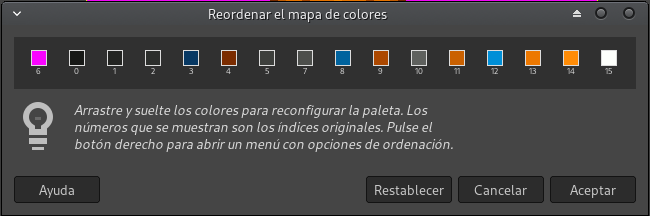
\includegraphics[width=0.6\textwidth]{archivos/paleta_map.png}
  \caption{Reordenar paleta de colores desde GIMP.}
  \label{fig:paleta_map}
\end{figure}

\vspace{0.5cm}

Por último, si compilamos el juego y lo ejecutamos, deberíamos tener algo como lo siguiente:

\clearpage

\begin{figure}[htbp]
\centering
  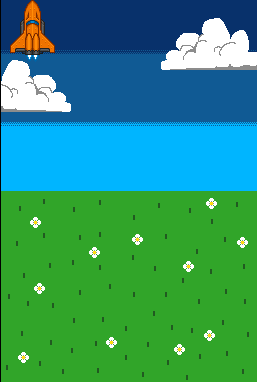
\includegraphics[width=0.3\textwidth]{archivos/sprite_prue.png}
  \caption{Prueba de dibujado de sprites.}
  \label{fig:sprite_prue}
\end{figure}

\subsubsection{Input}

Vamos a ver ahora cómo conocer y \textbf{gestionar la entrada del usuario}. Esta tarea es bastante más sencilla que lo anterior que hemos estado viendo gracias a libnds, que nos facilita el trabajo. Para gestionar todo esto haremos una función \textbf{handleInput} que deberá ser llamada una vez en cada iteración del programa.

\vspace{0.5cm}

En esta función llamaremos a la función \textbf{scanKeys()} de libnds. Esto hará que se \textbf{actualice el estado de todos los botones de la consola}, pantalla táctil incluída. Después, podemos llamar a la función de evento que queramos de entre tres: \textbf{keysHeld}, si queremos comprobar las teclas que están siendo presionadas continuamente, \textbf{keysDown}, las que se acaban de pulsar, y \textbf{keysUp}, las que se acaban de soltar.

\vspace{0.5cm}

Lo único que nos faltaría es especificar qué tecla queremos comprobar exactamente para ese evento. Para ello usaremos las máscaras de libnds.

\begin{lstlisting}[caption={Función para comprobar si el jugado mantiene pulsado el pad de direcciónes hacia abajo}, label={code:gameinput}]
void handleInput(){
	scanKeys();

	if (keysHeld() & KEY_DOWN){
        //ha pulsado la tecla
	}
\end{lstlisting}

\vspace{0.5cm}

\begin{table}[hbtp]
\centering
\begin{tabular}{|l|l|l|}
\hline
            & \textbf{Máscara de bit}            & \textbf{Botón de la consola}               \\ \hline
KEY\_A      & 1 \textless{}\textless 0  & A                                 \\ \hline
KEY\_B      & 1 \textless{}\textless 1  & B                                 \\ \hline
KEY\_SELECT & 1 \textless{}\textless 2  & Select                            \\ \hline
KEY\_START  & 1 \textless{}\textless 3  & Start                             \\ \hline
KEY\_RIGHT  & 1 \textless{}\textless 4  & Derecha (Pad de direcciones)      \\ \hline
KEY\_LEFT   & 1 \textless{}\textless 5  & Izquierda (Pad de direcciones)    \\ \hline
KEY\_UP     & 1 \textless{}\textless 6  & Arriba (Pad de direcciones)       \\ \hline
KEY\_DOWN   & 1 \textless{}\textless 7  & Abajo (Pad de direcciones)        \\ \hline
KEY\_R      & 1 \textless{}\textless 8  & R                                 \\ \hline
KEY\_L      & 1 \textless{}\textless 9  & L                                 \\ \hline
KEY\_X      & 1 \textless{}\textless 10 & X                                 \\ \hline
KEY\_Y      & 1 \textless{}\textless 11 & Y                                 \\ \hline
KEY\_TOUCH  & 1 \textless{}\textless 12 & Pantalla táctil (sin coordenadas) \\ \hline
KEY\_LID    & 1 \textless{}\textless 13 & Consola plegada                   \\ \hline
\end{tabular}
\caption{Máscaras de teclas.}
\label{table:gameinput}
\end{table}

\subsection{Iteración 1 - Pantallas del juego y lógica de los enemigos}

Una vez ya adquiridos los conocimientos y la práctica necesarios para programar los gráficos en la NDS, comencé a desarrollar el producto. 

\vspace{0.5cm}

Lo primero que quise implementar fueron las pantallas de juego, es decir, que de un menú principal pulsase una tecla y cargase un nivel. Para ello, primero hice un diagrama de clases que reflejan los distintos estados que tendría el juego.

\clearpage

\begin{figure}[htbp]
\centering
  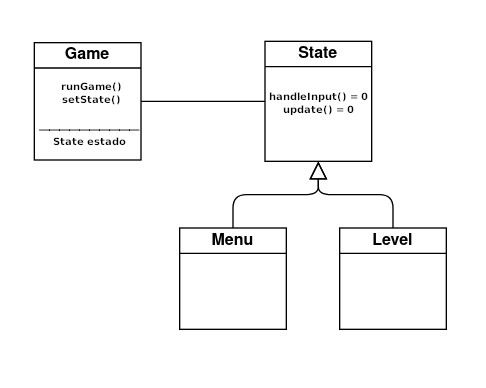
\includegraphics[width=0.6\textwidth]{archivos/state.png}
  \caption{Diagrama de los estados del juego y sus clases.}
  \label{fig:borrar}
\end{figure}


\vspace{0.5cm}

Como vemos en la anterior imágen, nuestra clase principal sería Game, que tendría un objeto de tipo State. Este sería el estado actual de juego, el cual al comienzo se inicializaría con el estado Menu. Menu y Level son dos clases que heredan de State, y ésta es una interfaz cuyos métodos virtuales son los típicos de un estado: handleInput() y update(). Así, todos los estados tendrán esos métodos pero los implementarán de forma distinta, por ejemplo, el handleInput() de Menu simplemente debe comprobar que se pulse una única tecla para comenzar el juego, mientras que el Level requiere de otros inputs y es más complejo. Toda esta implementación de estados cumple el patrón state de programación orientada a objetos.

\vspace{0.5cm}

Por otro lado, para que los estados fuesen accesibles desde muchos contextos (por ejemplo, desde la futura clase player cuando muera querrá llamar a que se cambie al estado GameOver) estos debían ser únicos. Para ello, todos los estados tendrían un método Instance(), que devuelve un puntero al objeto de ese tipo de estado. Pero ¿cómo asegurarnos de que solo existe un único objeto de cada estado? Esto lo haremos mediante una variable estática.

\vspace{0.5cm}

\begin{lstlisting}[caption={Implementación del patrón Singleton}, label={code:singleton}]

Level* Level::Instance(){
	static Level pinstance;
	return &pinstance;
}

\end{lstlisting}

\vspace{0.5cm}

Como podemos ver en el anterior código, en cada método Instance() de cada estado habrá una variable estática del tipo del estado. Una variable estática se crea al principio del programa y su vida es toda la ejecución de éste hasta que acaba. Es decir, que la variable pinstance se inicializará la primera vez que nosotros llamemos a ese método, creando así un objeto del tipo del estado, pero cuando volvamos a llamarla ésta ya estará creada así que simplemente nos la devuelve sin volver a crear una nueva. Esto en cuanto a diseño, es conocido como patrón Singleton.

\vspace{0.5cm}

También creé una clase Graphics, que se encargaría de realizar todas las tareas gráficas. Esto es para abstraer de la lógica del juego todas las funciones de libnds y hacer así un código más límpio. Esto en cuanto a diseño, es conocido como patrón Facade, pues la clase Graphics serviría a modo de fachada entre libnds y nuestro juego. Así, si en un futuro deseamos cambiar la librería es mucho más sencillo de hacer.

\vspace{0.5cm}

Por último, lo que hice durante esta iteración fue la gestión de un array de enemigos. Estos enemigos se crean al principio para evitar reservar memoria durante el juego, pero están inactivos. Para que fuesen saliendo uno a uno, creé un reloj que, al llegar a 0, recorre dicho array de enemigos buscando el siguiente inactivo para activarlo. Una vez están activos, estos enemigos se empiezan a mover hacia la derecha hasta el centro de pantalla.

\vspace{0.5cm}

\begin{figure}[htbp]
\centering
  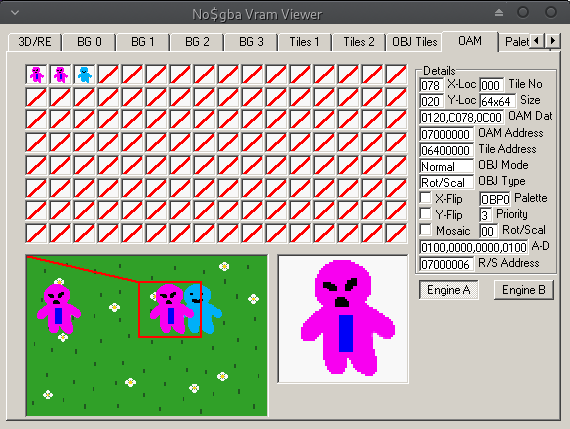
\includegraphics[width=0.6\textwidth]{archivos/borrar.png}
  \caption{Resultado de la ejecucion y elementos gráficos vistos desde el OAM Viewer de no\$gba}
  \label{fig:borrar}
\end{figure}

\subsection{Iteración 2 - Mecánicas y primera versión del algoritmo de reconocimiento de gestos}

En esta segunda iteración, me centré en el jugador y en el algoritmo de reconocimiento de gestos.

\vspace{0.5cm}

En cuanto al jugador, creé una clase Player que tiene variables como la vida, posición, etc. Para la vida, hice que los enemigos cada vez que colisionasen con el jugador redujesen la vida de este. También creé la vida del jugador, de la siguiente manera:

\vspace{0.5cm}

\begin{lstlisting}[caption={Implementación del patrón Singleton}, label={code:singleton}]

//create the life sprites
for(int i=0; i < MAX_LIFES; i++){
		p->setHeartSpriteId(i,g->createLifeSprites(0+(i*16),0));
}
\end{lstlisting}

\vspace{0.5cm}

Como podemos ver, el jugador tiene un número máximo de vidas (6). Este trozo de código lo que hace es ir creando los sprites de corazones para que la vida sea visible, pero al tener distinta posición en x, cada vez que crea uno se va aumentando. Esto hará que se creen corazones pegados uno al lado del otro.

\vspace{0.5cm}

Otra cosa a la que le dediqué tiempo fue a una primera versión del algoritmo de reconocimiento de gestos. Al principio solo quería distinguir entre una línea horizontal y otra vertical, así que lo que se me ocurrió fue guardarme la primera vez que toca la pantalla y la última. Para comprobar si esta era una línea horizontal restaba sus valores en X y si estos eran mayores de un umbral significaba que era una línea horizontal, y lo mismo para la vertical. Sin embargo, esto no funcionaba del todo correcto, pues las líneas inclinadas cumplían ambas condiciones.

\vspace{0.5cm}

Dejé esto de lado de momento e hice que los enemigos tuviesen un patron, así, al dibujar una línea se comprobaría si esa línea corresponde con el patrón del enemigo y, si es así, lo mataría.

\vspace{0.5cm}

Por último, lo que se realizó durante esta iteración fueron los sprites finales tanto de los enemigos como el jugador. Realicé el boceto en Procreate y el pixelart en GIMP.

\vspace{0.5cm}

\begin{figure}[htbp]
\centering
  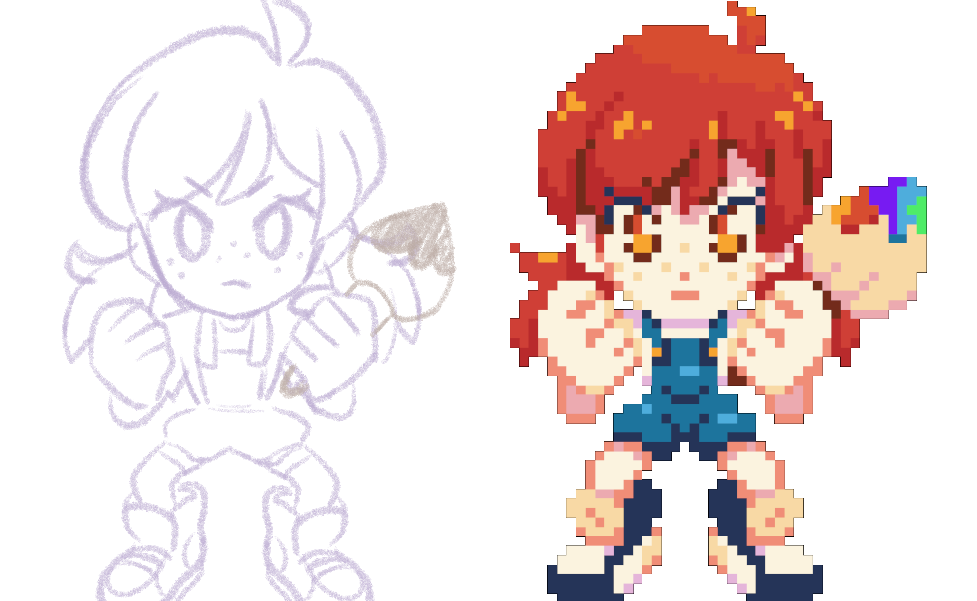
\includegraphics[width=0.6\textwidth]{archivos/sprite_player.png}
  \caption{Boceto y acabado del sprite del jugador}
  \label{fig:sprite_player}
\end{figure}

\vspace{0.5cm}

\begin{figure}[htbp]
\centering
  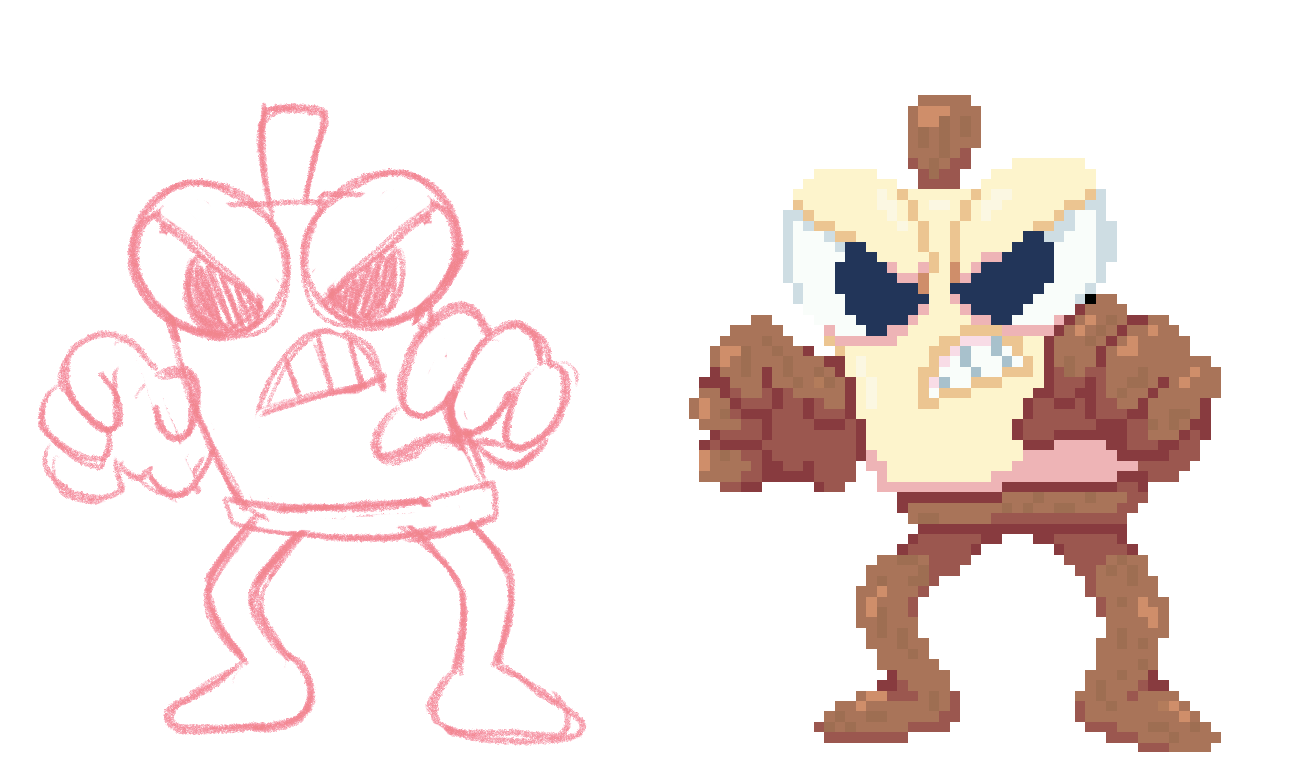
\includegraphics[width=0.6\textwidth]{archivos/sprite_enemy.png}
  \caption{Boceto y acabado del sprite del enemigo}
  \label{fig:sprite_enemy}
\end{figure}

\subsection{Iteración 3 - Algoritmo de reconocimiento de gestos}

En esta iteración quería centrarme en el desarrollo de un algoritmo de reconocimiento de gestos, pues era algo vital para la jugabilidad del proyecto.

\vspace{0.5cm}

Así pues, lo primero que hice fue pensar en qué necesitaría para poder comparar dos trazos, uno ideal y otro que fuese el que el usuario ha dibujado. Basándome en el algoritmo Graffiti, decidí que lo que debía hacer era guardar cada par de coordenadas que el usuario pulsaba mientras dibujaba un trazo en una estructura del tipo array. Para ello, primero pensé en crear una estructura llamada Vector2D, que almacena en ella dos enteros, la coordenada x y la y. Después, decidí usar como array std::vector, por varias razones. La primera es que para poder guardar una colección de pares de números que el usuario va introduciendo en tiempo de ejecución necesitaremos una estructura dinámica, pues algunos usuarios dibujan el trazo más lento, lo que implica más muestras y viceversa. Por otro lado, esta herramienta nos ofrece datos y funciones mu cómodas para trabajar con ella (funciones para insertar números, acceso a su tamaño y capacidad actuales, redimensionado...).

\vspace{0.5cm}

Empecé entonces por desarrollar la entrada del usuario. Para ello, me creé un proyecto aparte con el fin de probar este algoritmo en una pantalla con salida de texto para depurar, a diferencia de nuestro proyecto que ya tenía las pantallas con sus fondos ya cargados y cambiarlo supondría mucho trabajo.

\vspace{0.5cm}

\begin{lstlisting}[caption={Función consoleInit con los parámetros adecuados para crear un fondo que nos sirva para depurar}, label={code:consoleinit}]

    [...]
    
    /*Parámetros: 
    0: Puntero a la terminal que usa
    0: Capa de fondo que usa
    BgType_Text4bpp:	Tipo de fondo
    BgSize_T_256x256: tamanyo del fondo
    31: Comienzo en memoria
    0: 
    false: Usa el motor de la pantalla inferior (si es verdadero usa la superior)
    true:	Carga la fuente por defecto para ser usada*/

	consoleInit(0, 0,BgType_Text4bpp, BgSize_T_256x256, 31,0, false, true);
	
	[...]
	
	//17: Fila donde comenzar a escribir
	//5H: Columna donde comenzar a escribir
	printf("\x1b[17;5H Linea Vertical \n");
	
	[...]

\end{lstlisting}

\vspace{0.5cm}

El código anterior muestra cómo preparé la consola para poder mostrar mensajes por pantalla que me sirviesen de sistema de depuración.

\vspace{0.5cm}

Para insertar los valores del usuario, como ya vimos anteriormente en el apartado de Input en nuestra función handleInput() llamaremos primero a scanKeys() y touchread() par que nos actualice el estado actual de todos los botones incluyendo la pantalla táctil. Después, si el usuario está pulsando la pantalla deberemos distinguir dos casos: si es la primera ves que pulsa o no. Para ello, comprobaremos el tamaño del vector. Si este es menor de 1 significa que es la primera vez que pulsa y si no, ya lleva manteniendo pulsado un rato. Esto lo hago para poder ahorrarme introducir un par de valores nuevos en el array si estos son iguales al anterior.

\vspace{0.5cm}

\begin{lstlisting}[caption={Inserción de valores que conforman el trazo}, label={code:push_back}]

	[...]
	
	if(keysHeld() & KEY_TOUCH){
		
		//Guardamos el punto en el array
		if(pattern.size()>1){ //si lleva un rato pulsando

			auto* v = pattern[pattern.size()-1]; //nos guardamos el punto anterior (el ultimo)

			if(v->getX() != stylus.px || v->getY() != stylus.py){ //y lo comprobamos para que no sea igual al que vamos a introducir
				Vector2D* pos = new Vector2D(stylus.px, stylus.py);
				pattern.push_back(pos);
				pos = nullptr;
			}

			v = nullptr;

		}else{ //si es la primera vez que pulsa
			Vector2D* pos = new Vector2D(stylus.px, stylus.py);
			pattern.push_back(pos);
			pos = nullptr;
		}
		
	}
	
	[...]

\end{lstlisting}

\vspace{0.5cm}

Una vez hecho esto, cuando detectemos que el jugador deja de pulsar con la funcion keysUp() y la macro KEY\_TOUCH, tendríamos todas las coordenadas almacenadas y listas para trabajar con ellas.

\vspace{0.5cm}

Ahora bien, ¿cómo podemos comparar los dos trazos (ideal y del usuario) para saber si son parecidos? Matemáticamente podemos usar la desviación estándar, ya que tenemos un conjunto de valores y queremos ver su dispersión frente a los ideales. Esta desviación, a la que llamaremos $\sigma$ , se calcula con la media cuadrática de los valores o RMS (del inglés root mean square), de la siguiente forma:

\vspace{0.5cm}

\begin{equation}
x_{RMS} = \sqrt{\frac{1}{N}\sum_{i = 1}^{N} x_{i}^{2}}=\sqrt{\frac{x_{1}^{2} + x_{2}^{2} + x_{3}^{2} + ... + x_{N}^{2}}{N}}
\end{equation}

\vspace{0.5cm}

Así pues, cuanto menor sea $\sigma$, más se parecerán ambos trazos pues su desviación entre los puntos es menor.

\vspace{0.5cm}

Durante la ejecución del algoritmo lo que haremos será ir punto por punto calculando dicha desviación del punto ideal con el del usuario, acumulando todas las desviaciones para tener finalmente una desviación total que indicará cuánto se asemejan ambos patrones. Debemos tener en cuenta que estos cálculos los haremos independientemente por cada eje, así pues computaremos las coordenadas x por una parte, dandonos una desviación en dicho eje, y lo mismo con el eje y, sumando finalmente dichas desviaciones. Así pues, los cálculos que haremos por cada punto son los siguientes:

\vspace{0.5cm}

Para el eje X:
\begin{equation}
\sigma _{xn_{ideal}\rightarrow xn_{usuario}} = \sqrt{\frac{xn_{ideal}^{2} + xn_{usuario}^{2}}{2}}
\end{equation}

\vspace{0.5cm}

Para el eje Y:
\begin{equation}
\sigma _{xn_{ideal}\rightarrow xn_{usuario}} = \sqrt{\frac{xn_{ideal}^{2} + xn_{usuario}^{2}}{2}}
\end{equation}

\vspace{0.5cm}

Ahora bien, si bien calculando esto nos puede dar unos valores bastante fiables, hay un aspecto que tenemos que tener en cuenta primero.

\vspace{0.5cm}

El usuario, aunque por lo general dibujará el patrón lo más centrado que pueda, pero es posible que a veces al hacerlo rápido lo dibuje con tendencia a uno de los bordes de la pantalla. Por eso, si un patrón dibujado está muy desplazado con respecto al que debería ser al hacer el cálculo de la desviación esta puede aumentar, habiendo el riesgo de que entonces el algoritmo no te de el resultado correcto. Para solventar esto, he elegido como punto de referencia el inicio del trazo, tal y como hace Graffiti, y he añadido que por cada punto le reste la distancia tanto en x como en y para desplazar todo el trazo. Esto se muesra mejor en la siguiente figura:

\vspace{0.5cm}

\begin{figure}[htbp]
\centering
  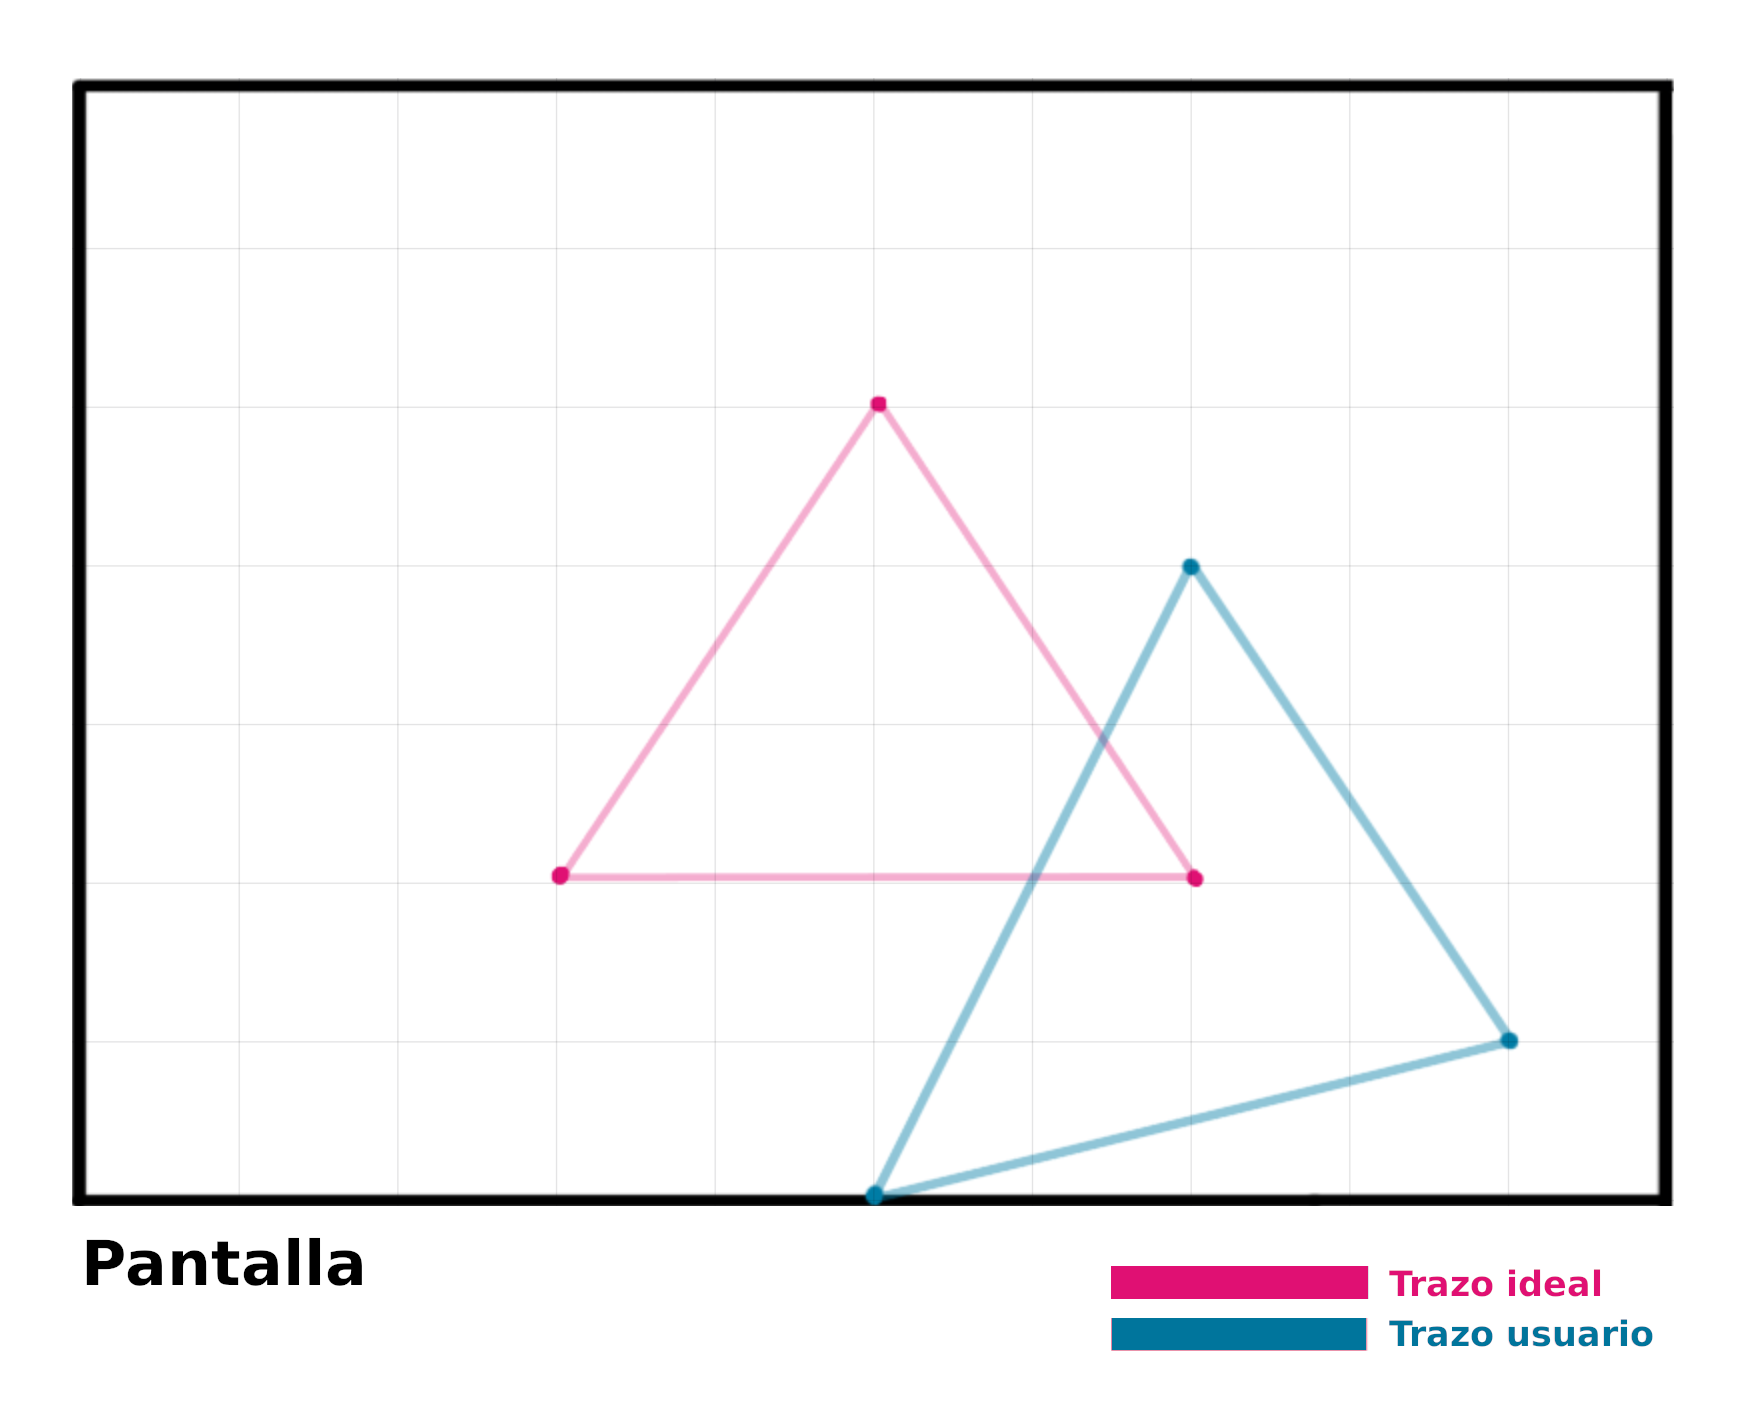
\includegraphics[width=0.6\textwidth]{archivos/shape_not_displaced.png}
  \caption{Visualización del trazo ideal y del usuario sin aplicar el desplazamiento}
  \label{fig:shape_not_displaced}
\end{figure}

\clearpage

\begin{figure}[htbp]
\centering
  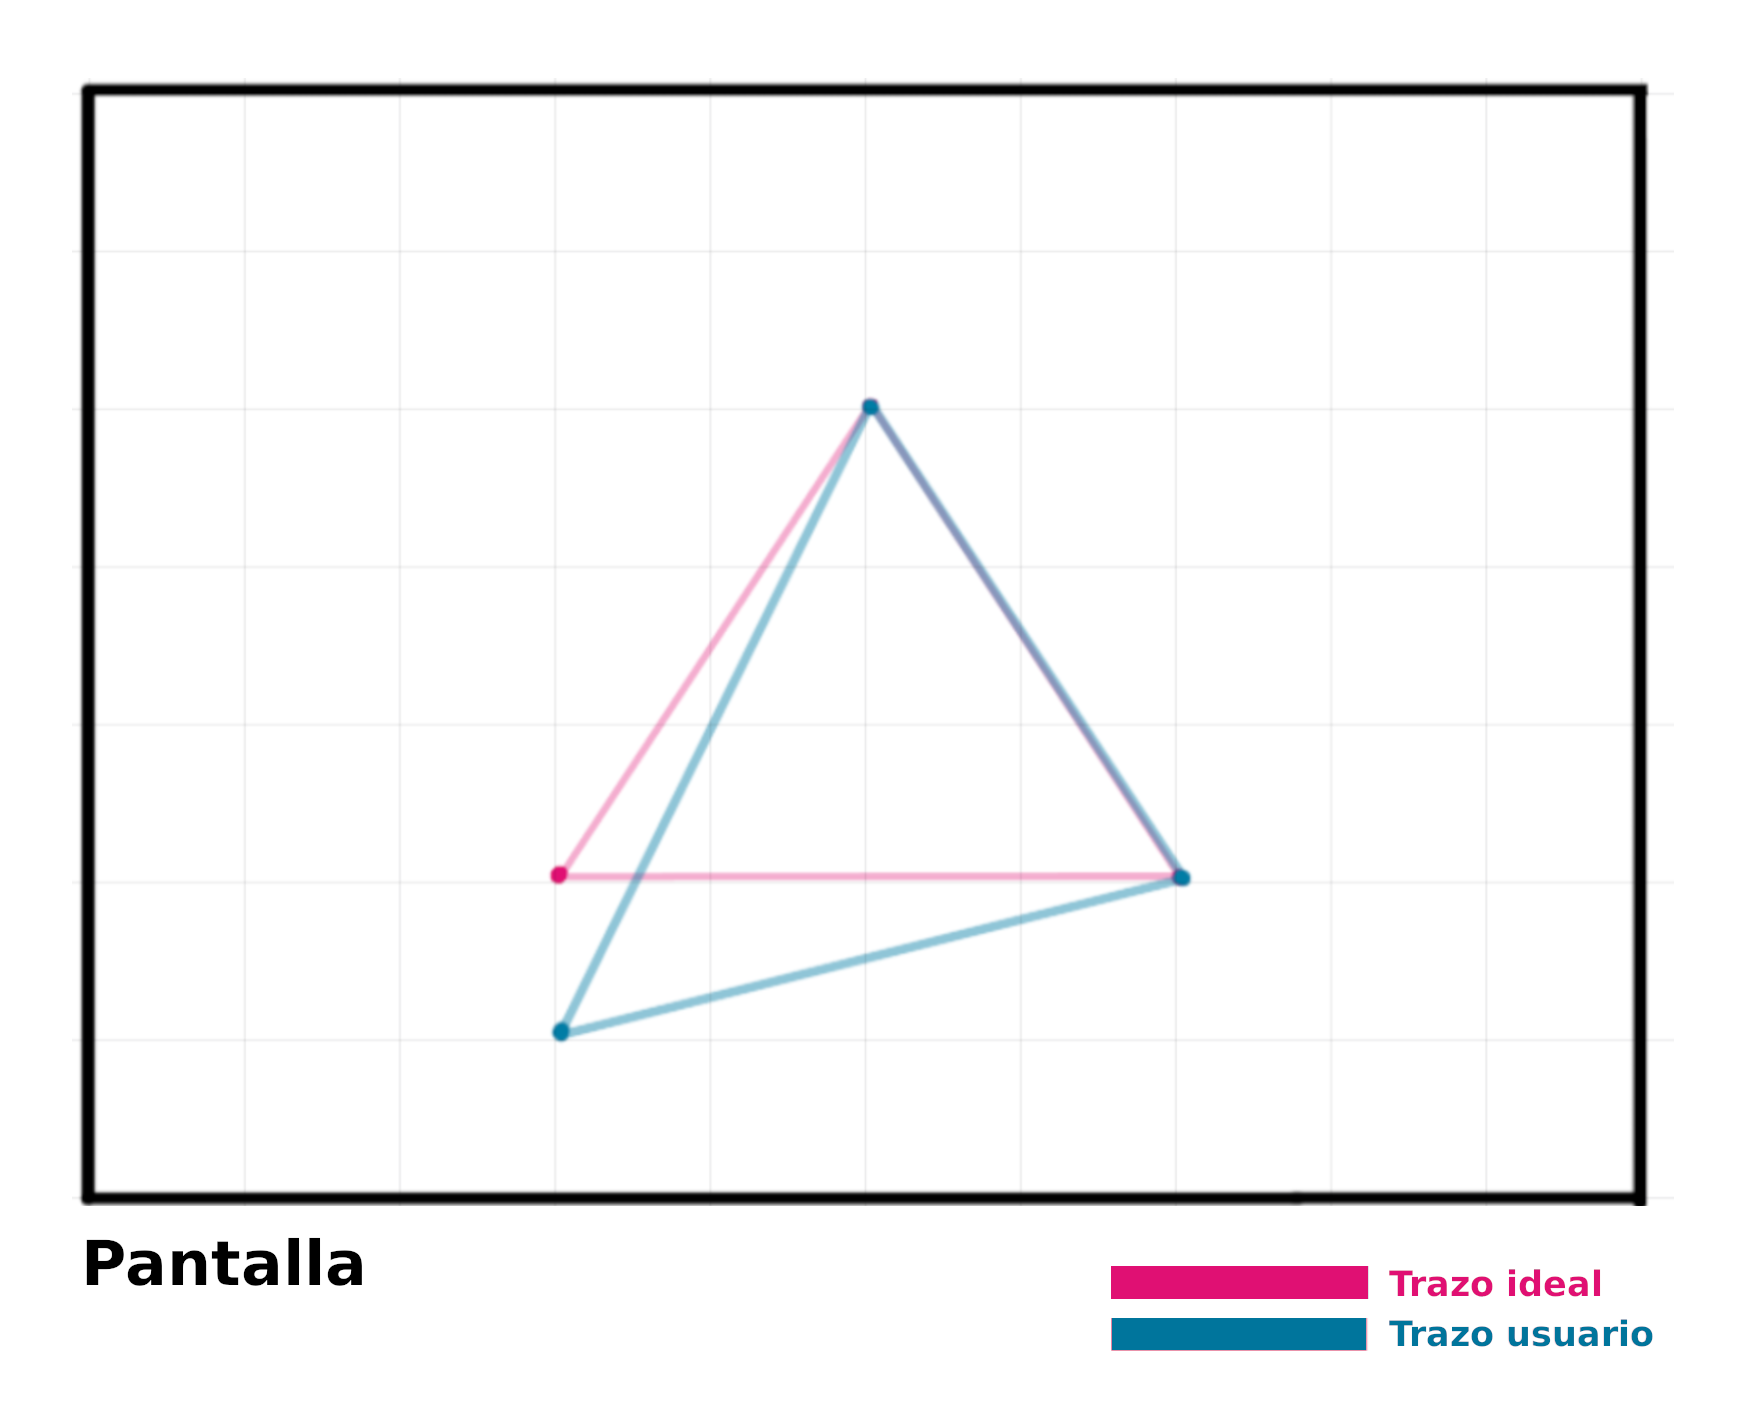
\includegraphics[width=0.6\textwidth]{archivos/shape_displaced.png}
  \caption{Visualización del trazo ideal y del usuario con el desplazamiento aplicado}
  \label{fig:shape_displaced}
\end{figure}

\vspace{0.5cm}

Las fórmulas entonces de estos desplazamientos serían las siguientes:

\vspace{0.5cm}

\begin{equation}
dx =x1_{ideal} - x1_{usuario}
\end{equation}

\vspace{0.5cm}

\begin{equation}
dy =y1_{ideal} - y1_{usuario}
\end{equation}

\vspace{0.5cm}

Y esto es todo lo que deberíamos tener en cuenta, así que el algoritmo sería el siguiente:

\vspace{0.5cm}

\begin{lstlisting}[caption={Algoritmo de reconocimiento de gestos}, label={code:checkpattern}]
float checkPattern(const Vector2D shape[]){

	//calcule displacement in both axis
	//of the user pattern from the ideal pattern
	int dx,dy;

	Vector2D s = shape[0];
	Vector2D* u = pattern[0];

	dx = s.getX() - u->getX();
	dy = s.getY() - u->getY();


	//user pattern iterator
	float inc = (pattern.size()-1)/(ANCHOR_POINTS-1);
	float j = 0.0;


	//total deviation 
	float o_tot = 0.0;

	for(int i=0;i<ANCHOR_POINTS;i++){

		u = pattern[j];
		s = shape[i];

		//displace point
		int x_ = u->getX() + dx;
		int y_ = u->getY() + dy;


		//Calculate RMS and deviation for x and y
		float rms_x, rms_y, aux;
		aux = 0.0;

		//x coordinate
		aux = pow(s.getX(),2) + pow(x_,2);            // x1² + x2²
		aux = aux/2.0;								                      // ---------
                                                                                        //     2
		rms_x = sqrt(aux);

		o_tot = o_tot + abs(s.getX() - rms_x);
		

		//y coordinate
		aux = pow(s.getY(),2) + pow(y_,2);             // y1² + y2²
		aux = aux/2.0;								                        // ---------
                                                                                          //     2   
		rms_y = sqrt(aux);

		o_tot = o_tot + abs(s.getY() - rms_y);


		if(i == ANCHOR_POINTS-1){
			j = pattern.size();
		}else{
			j = j + inc;
		}

	}

	return o_tot;

}
\end{lstlisting}

\vspace{0.5cm}

La variable ANCHOR\_POINTS se trata de una macro que establece cuántos puntos de muestra se usan para trabajar con el algoritmo, al igual que hace el algoritmo de PAlib. Esto hace que la velocidad del algoritmo sea mayor, aunque también aumenta el error.

\vspace{0.5cm}

Por último, una vez introducidos los datos de los patrones ideales, el algoritmo funcionaba correctamente como se ve en la siguiente imágen:

\vspace{0.5cm}

\begin{figure}[htbp]
\centering
  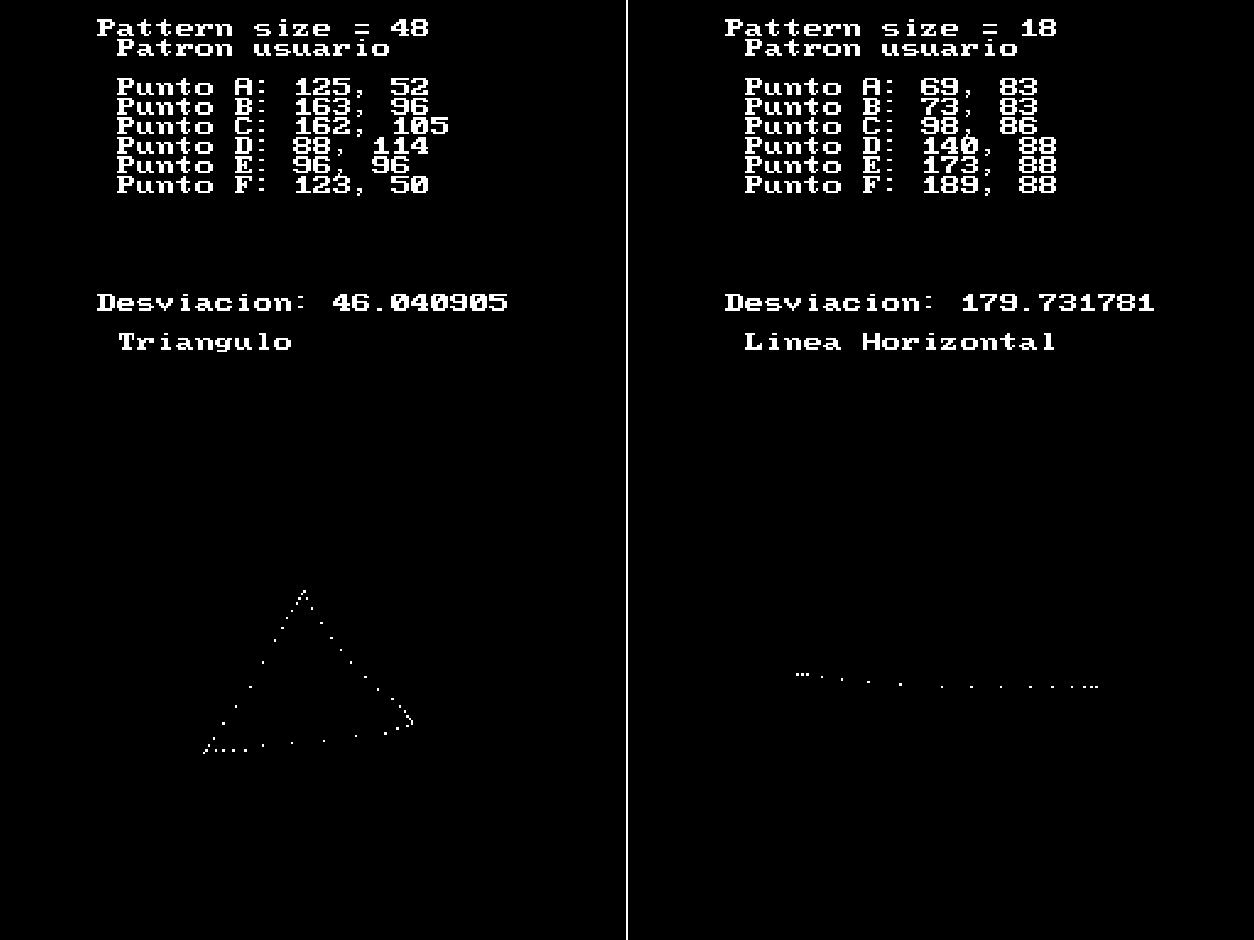
\includegraphics[width=0.8\textwidth]{archivos/pattern_test_1.png}
  \caption{Resultado de la prueba del algoritmo desarrollado probando}
  \label{fig:pattern_test_1}
\end{figure}

\clearpage

\begin{figure}[htbp]
\centering
  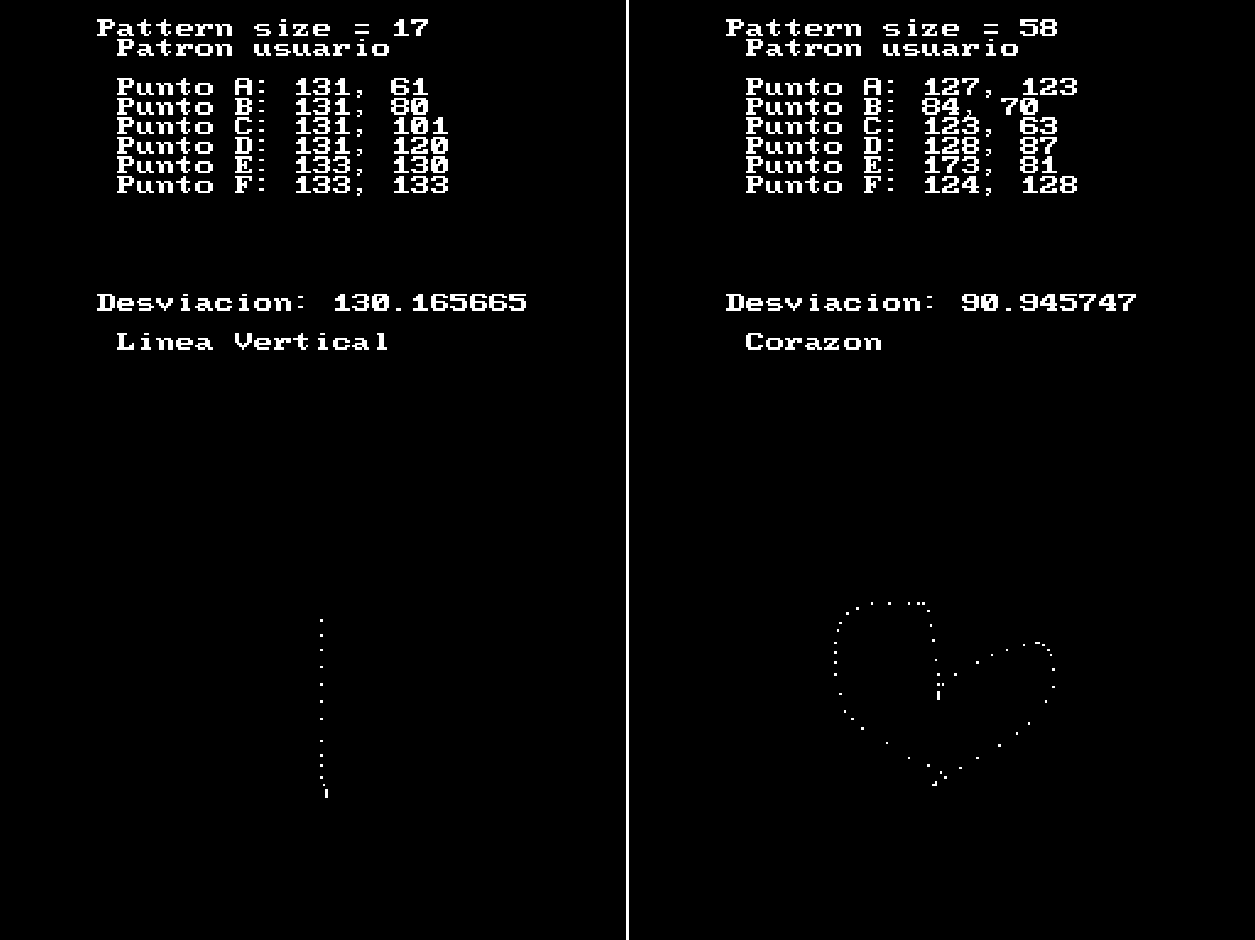
\includegraphics[width=0.8\textwidth]{archivos/pattern_test_2.png}
  \caption{Resultado de la prueba del algoritmo desarrollado probando}
  \label{fig:pattern_test_2}
\end{figure}

\vspace{0.5cm}

\subsection{Iteración 4 - Jugabilidad y ajustes de aparición de enemigos}

Durante esta iteración me centré en avanzar en la parte jugable del juego, es decir en las mecánicas y niveles.

\vspace{0.5cm}

Lo primero en lo que me centré fue en el dibujado en la pantalla táctil para que el usuario pudiese ver de una manera agradable lo que estaba pintando. Así pues, quise conseguir un efecto similar al que tiene el juego Wario Ware: Touched! en su pantalla de inicio.

\vspace{0.5cm}

En esta pantalla, aparecen un montón de elementos casi aleatoriamente y, de vez en cuando, aparece una pelota que el usuario puede arrastrar y al moverse crea un rastro verde que desaparece con el tiempo.

\clearpage
\begin{figure}[htbp]
\centering
  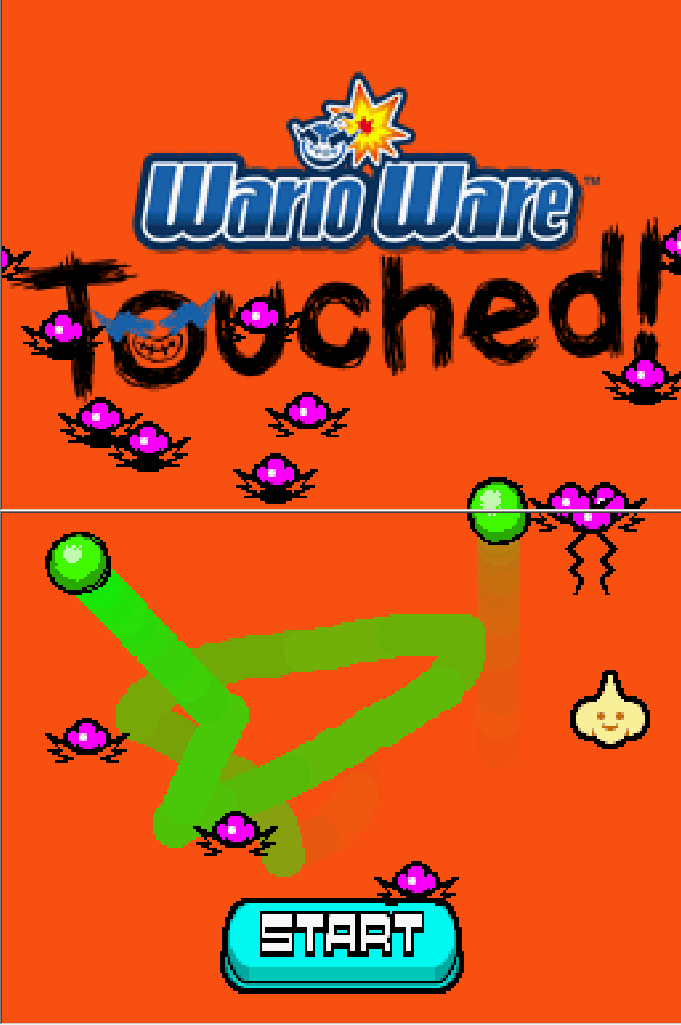
\includegraphics[width=0.4\textwidth]{archivos/wario_ware_draw.png}
  \caption{Pantalla de inicio de Wario Ware: Touched!}
  \label{fig:warioware_main_creen}
\end{figure}

\vspace{0.5cm}

Mi idea era parecida a esto, solo que quería que el rastro fuese permanente hasta que el usuario dibujase el patrón por completo y quería además que dicho rastro fuese con muchos colores, como si se tratase de un arcoíris para dar la sensación de que estuvieses dibujando con un pincel mágico.

\vspace{0.5cm}

Para implementar esto rápidamente se me ocurrió una idea, pues como ya he comentado, por cada pantalla somos capaces de dibujar hasta 4 fondos y estos pueden tener un color de transparencia. Así pues, mi idea era dibujar un fondo con degradado de arcoíris, encima de este otro simulando un lienzo y, por cada pixel que el usuario tocase en la pantalla táctil, pintar el color transparente en el fondo superior para que dejase ver el inferior.

\vspace{0.5cm}

Así pues, comencé por dibujar los dos fondos en la pantalla táctil, lo cual ya me causó problemas. Para mapear la memoria de vídeo como memoria de fondos, asigné el banco C usando la instrucción vramSetBankC(VRAM\_C\_SUB\_BG\_0x06200000). De este modo tenemos 128 kilobytes disponibles para memoria de fondos, lo cual es suficiente para lo que necesitamos.

\vspace{0.5cm}

Para dibujar los fondos, como ya he comentado anteriormente primero incialicé los registros controladores de los fondos.

\vspace{0.5cm}

\begin{lstlisting}[caption={Configuración de los registros controladores de los fondos de la pantalla inferior}, label={code:subbgconfig}]

    //set control registrers for canvas background on the sub screen
    //                                           Size of the bg  |   Initial position in memory  | priority (higher so appears on top)
    REG_BG3CNT_SUB = BG_BMP16_256x256 | BG_BMP_BASE(0) | BG_PRIORITY(2);

    //affine matrix of the background
    REG_BG3PA_SUB = 1 << 8;  REG_BG3PC_SUB = 0;
    REG_BG3PB_SUB = 0;       REG_BG3PD_SUB = 1 << 8;

    //position of the background
    REG_BG3X_SUB = 0;
    REG_BG3Y_SUB = 0;

    //set control registrers for the rainbow background on the sub screen
    REG_BG2CNT_SUB = BG_BMP8_256x256 | BG_BMP_BASE(8) | BG_PRIORITY(3);

    //affine matrix of the background
    REG_BG2PA_SUB = 1 << 8;  REG_BG2PC_SUB = 0;
    REG_BG2PB_SUB = 0;       REG_BG2PD_SUB = 1 << 8;

    //position of the background
    REG_BG2X_SUB = 0;
    REG_BG2Y_SUB = 0;

\end{lstlisting}

\vspace{0.5cm}

Sin embargo, al ejecutar el juego no conseguía ver el fondo superior. Pasé un rato analizando qué estaba ocurriendo, pues a pesar de que estaba copiando donde esperaba el fondo, no se visualizaba ni en el juego, ni en las ventanas de depuración de no\$gba. Al final, opté por usar una herramienta que me ayudaría a verificar si lo que estaba intentando hacer tenía o no sentido.

\vspace{0.5cm}

Dicha herramienta es un visualizador de conflictos de asignación de VRAM para fondos en un navegador\footnote{https:\/\/mtheall.com\/vram.html\#}. En ella puedes introducir las configuraciones de tus fondos (tamaño, profundidad y posicion inicial en memoria), la pantalla en la cual vas a dibujar los fondos y te proporciona si se van a producir conflictos e incluso qué bancos deberías usar. Pues bien, introducidos los datos de mi configuración dió el resultado de la figura 5.22.

\vspace{0.5cm}

\begin{figure}[htbp]
\centering
  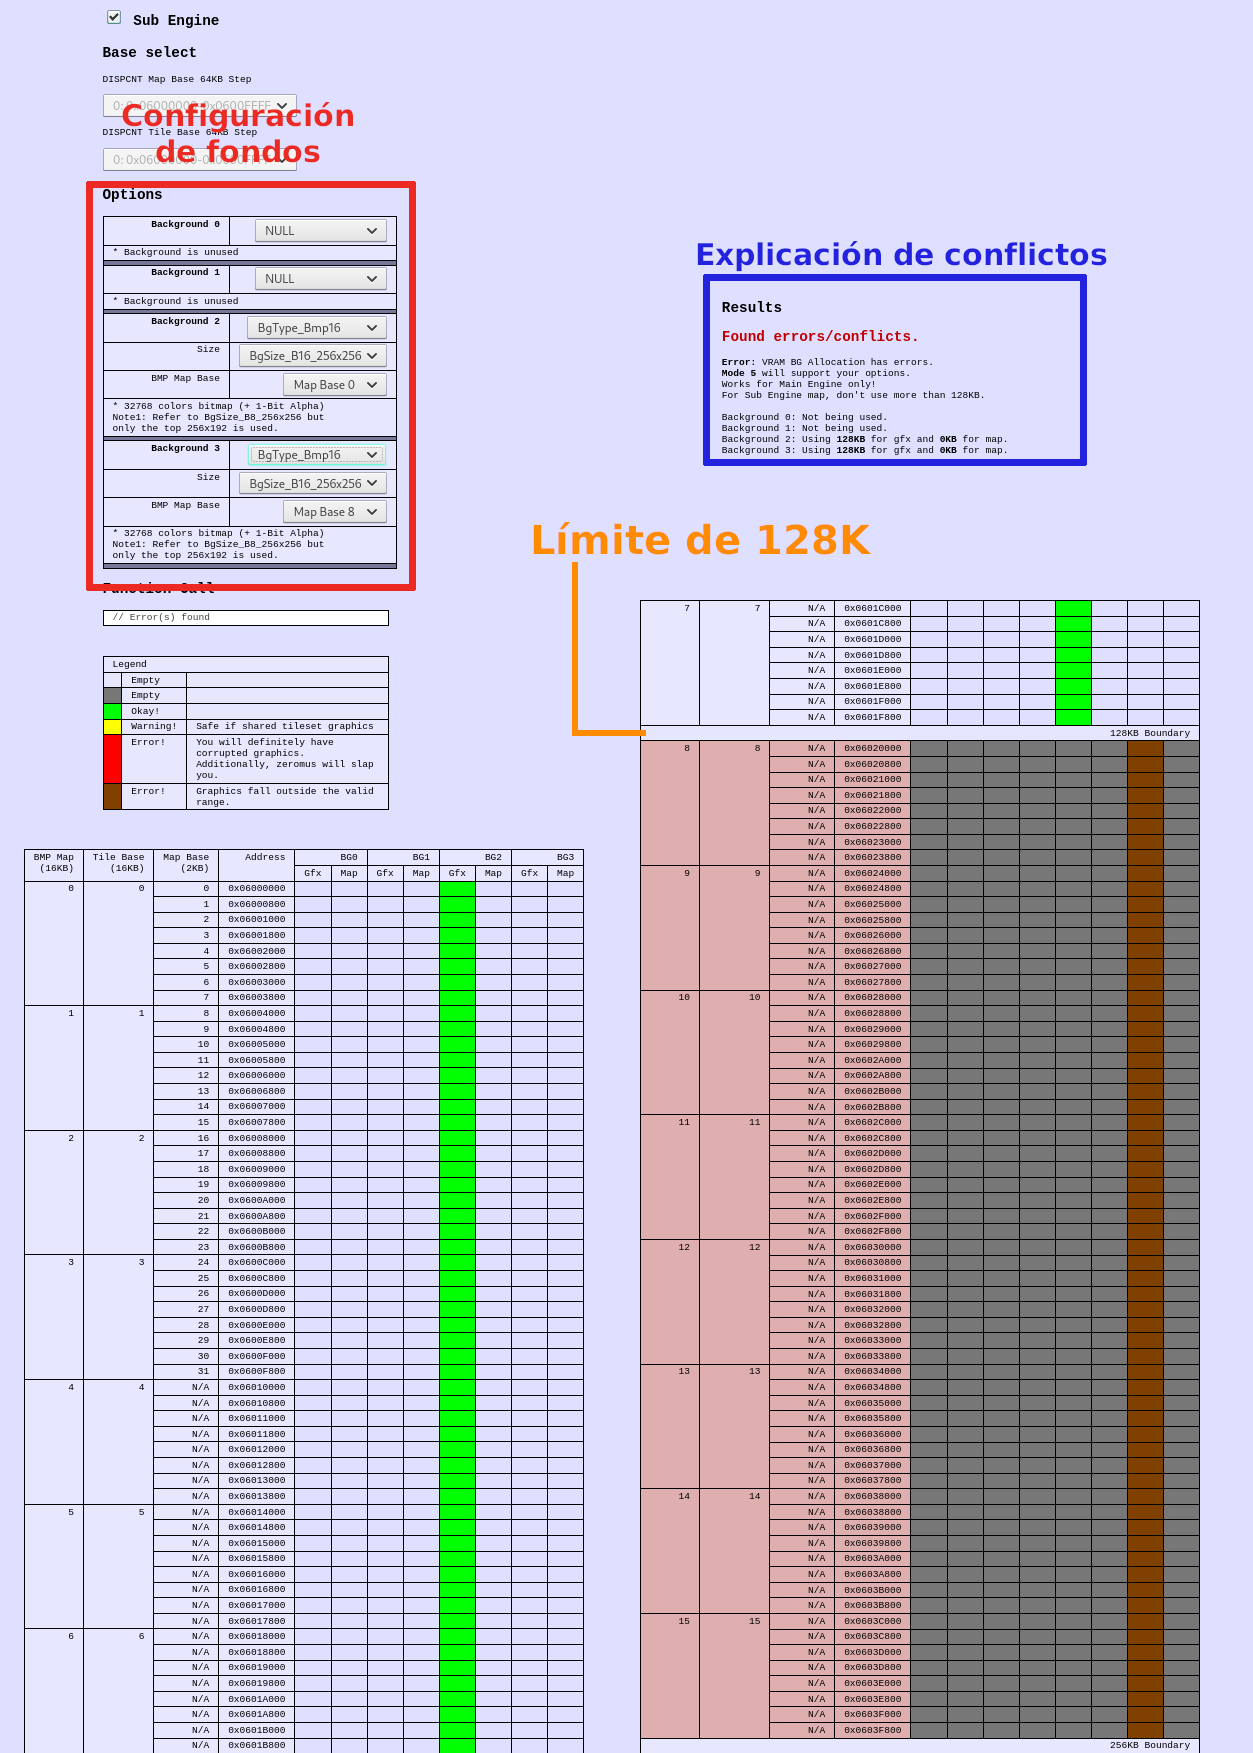
\includegraphics[width=0.9\textwidth]{archivos/vram_allocator.png}
  \caption{Resultado de la consulta con la mala configuración de fondos}
  \label{fig:vram_allocator_problem}
\end{figure}

\vspace{0.5cm}

Fué ahí entonces cuando entendí lo que estaba pasando. Con la configuración actual, un solo fondo ocupaba todo el espacio disponible (los 128KB) de memoria de vídeo, y el siguiente se quedaba fuera del banco, con lo cual no se iba a ver nunca. Para solucionar esto, cambié los fondos para que tuviesen una profundidad de 8 bits por pixel, en lugar de 16 y así ambos cabrían en el espacio de memoria sin problemas, como muestra la siguiente figura.

\vspace{0.5cm}

\begin{figure}[htbp]
\centering
  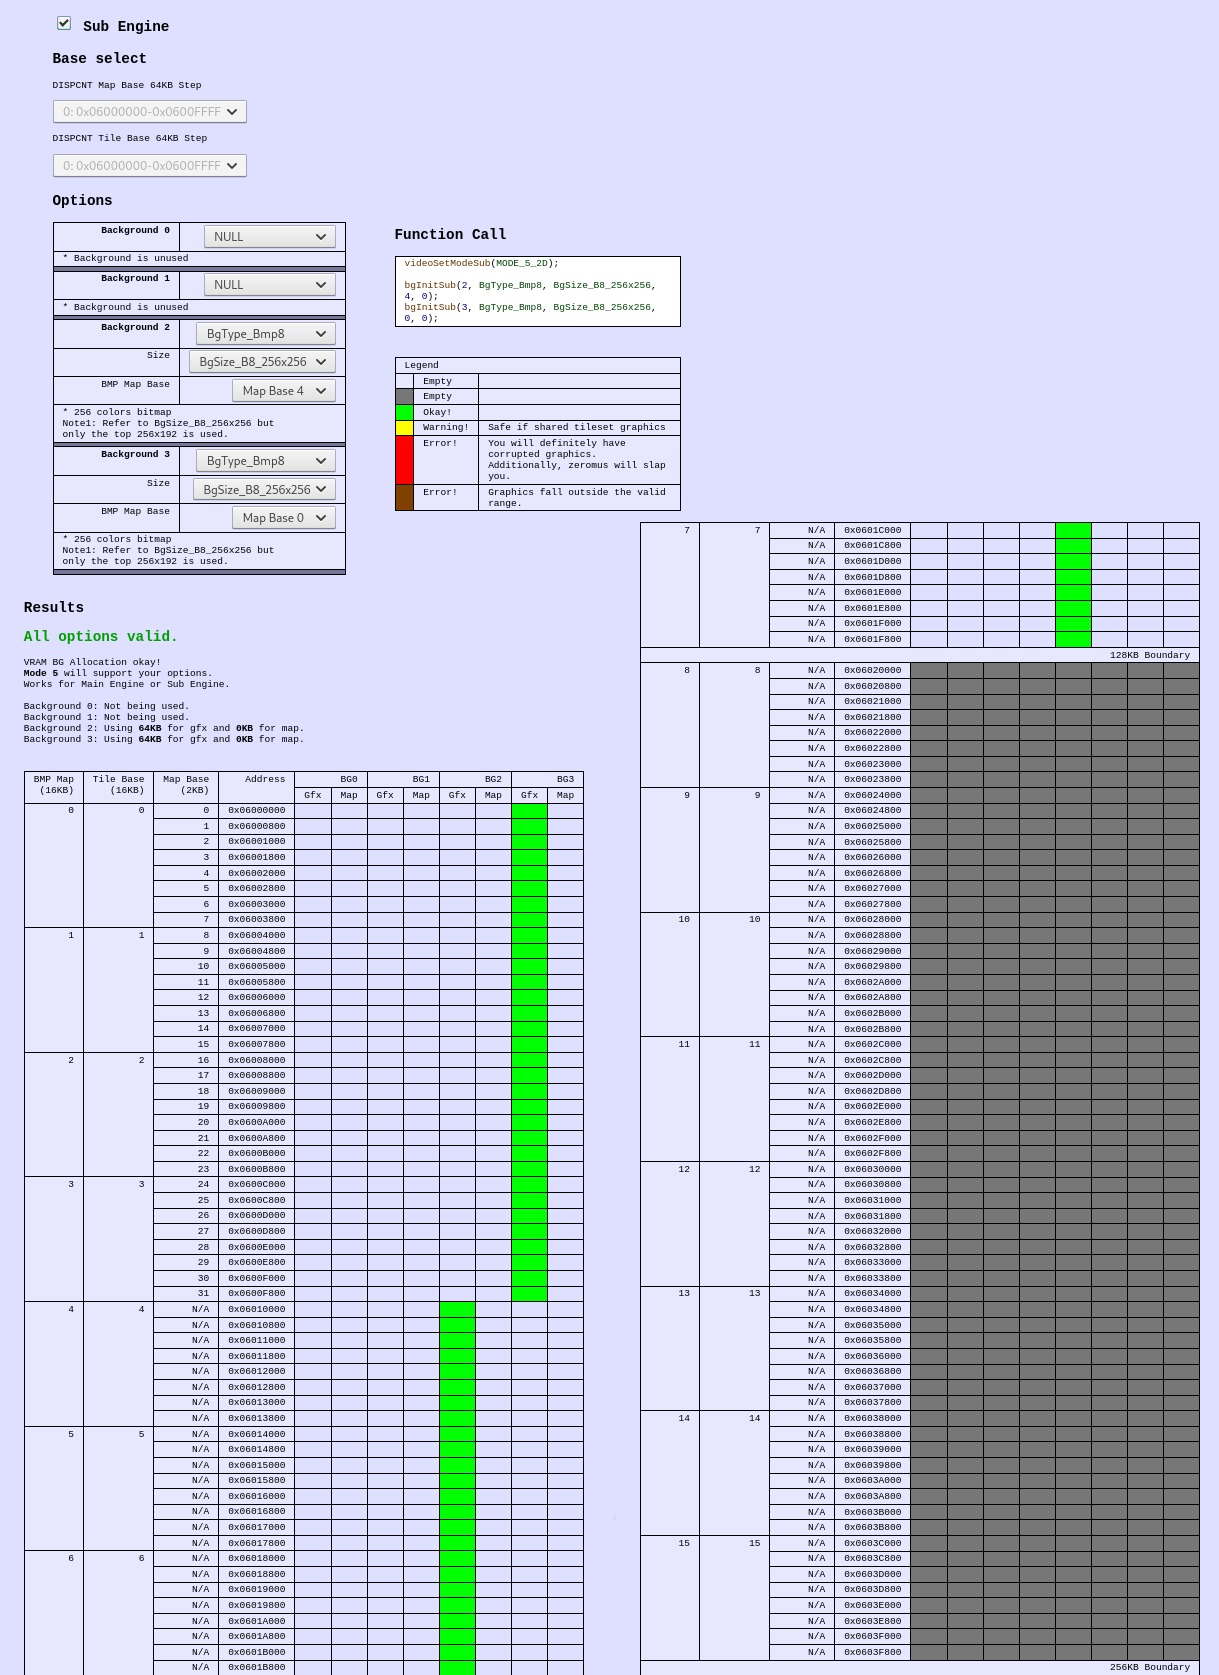
\includegraphics[width=0.9\textwidth]{archivos/vram_allocator_2.png}
  \caption{Resultado de la consulta con una buena configuración de fondos}
  \label{fig:vram_allocator_good}
\end{figure}

\vspace{0.5cm}

Los cambios que tuve que realizar para solucionar esto no supusieron gran complicación, simplemente cambiando los registros controladores de fondos de 16 a 8 bpp usando la macro BG\_BMP8\_256x256, también en los archivos de configuración de grit de cada fondo, especifiqué también la profundidad de pixel con el parámetro -gB8 y por último, como ambos fondos debían usar la misma paleta de X colores, abrí ambos fondos en GIMP y los exporté para que usaran la misma paleta de colores. Esto puede hacerse sencillamente abriendo ambos fondos en el mismo archivo de gimp, cambiando el modo de color a indexado y en el menú emergente seleccionar la opción de ''Generar paleta óptima" con 16 colores, como ya hemos comentado en otras ocasiones.

\vspace{0.5cm}

\begin{figure}[htbp]
\centering
  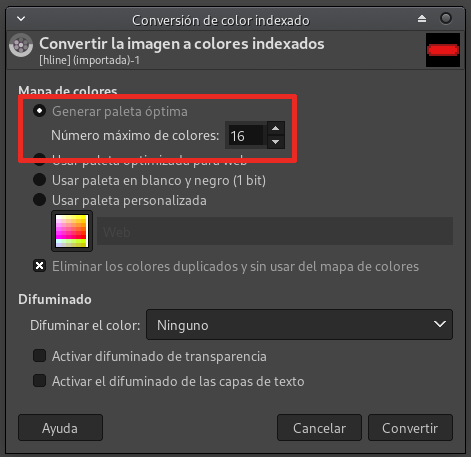
\includegraphics[width=0.4\textwidth]{archivos/gimp_indexed.png}
  \caption{Cambio de imágen a modo indexado y selección de paleta}
  \label{fig:gimp_indexed}
\end{figure}


\vspace{0.5cm}

También, otra cosa que tuve que tener en cuenta fué especificar dónde comenzaba el segundo fondo en memoria. Antes, usaba la macro BG\_BMP\_BASE(8) para indicar que el segundo fondo comenzaba en la dirección 0x06020000, lo cual ya hemos visto que se nos quedaba fuera del rango disponible. Sin embargo, ahora el primer fondo ocupa la mitad de espacio, acabando en la posición 0x0600FFFF, con lo cual podía copiar el segundo a partir de la posición 0x06010000. Para representar esto con dicha macro basta con pasarle por parámetro el número 4, pues indica que, de los 8 bloques (numerados del 0 al 7) de 16KB cada uno  en los que están divididos los 128KB de la memoria, el fondo comenzaría en el cuarto. Esto se puede ver gráficamente  en la figura anterior, fijándonos en la columna BMP Map.

\vspace{0.5cm}

Una vez hecho esto, ya conseguí que se viesen ambos fondos, no obstante, aún había un pequeño problema. Como se ve en la siguiente figura, en la esquina superior izquierda del fondo se ven unos colores grises que no deberían aparecer, pues en su lugar era un tono de rojo. Esto me hizo pensar que quizás había algún problema con las paletas, así que usé las herramientas de depuración de no\$gba para ver qué ocurría.

\clearpage

\begin{figure}[htbp]
\centering
  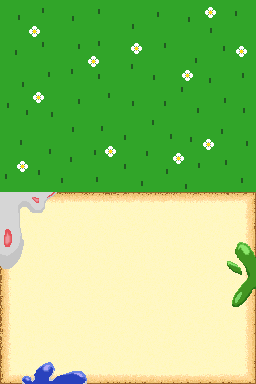
\includegraphics[width=0.4\textwidth]{archivos/background_gray.png}
  \caption{Fondo dibujado con un problema en la paleta}
  \label{fig:background_gray}
\end{figure}

\vspace{0.5cm}

Así pues, como se ve en la figura 5.26 vi que habían unos 48 colores en escala de grises que no parecían pertenecer a la paleta de los fondos, era como si se hubiesen copiado por encima de ésta. Sospeché que el problema venía de la zona de memoria donde se copian las paletas de los sprites, pues la zona de memoria consecutiva a ésta es precisamente la dedicada a paletas de fondos de la pantalla inferior. Al comprobar las paletas de sprites, vi que también estaba presente ese degradado en tonos grises, lo cual me indicaba más aún de que alguna de las paletas de los sprites había sobreescrito las de los fondos al salirse de los límites. Comprobé entonces todos los sprites y efectivamente, el sprite del jugador tenía una paleta de 256 colores, seguramente por un despiste al exportar el archivo desde GIMP. Arreglado esto ya se veía el fondo perfectamente.

\vspace{0.5cm}

\begin{figure}[htbp]
\centering
  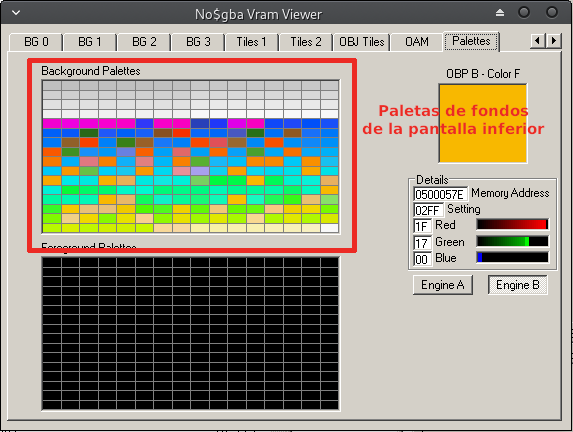
\includegraphics[width=0.6\textwidth]{archivos/palettes_bg_sub_overwritten.png}
  \caption{Superposición de tonos grises en la paleta de los fondos de la pantalla inferior}
  \label{fig:palettes_bg_sub_overwritten}
\end{figure}

\vspace{0.5cm}

\begin{figure}[htbp]
\centering
  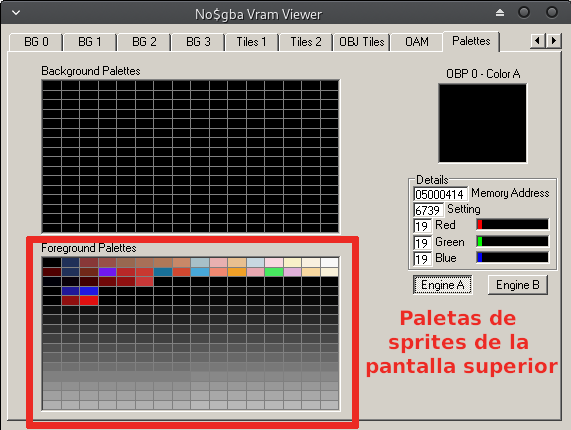
\includegraphics[width=0.6\textwidth]{archivos/palette_sprites_overflow.png}
  \caption{Paletas de los sprites que se salen de los límites}
  \label{fig:palette_sprites_overflow}
\end{figure}

\vspace{0.5cm}

Una vez tenía ambos fondos dibujados, lo siguiente que quería hacer era conseguir que al pulsar en la pantalla táctil en una coordenada (x,y), calcular dónde estaría ese pixel en memoria y cambiar ese pixel a negro ya que sería el color transparente, dejando así ver el fondo de arcoíris que está debajo de él.

\vspace{0.5cm}

\begin{figure}[htbp]
\centering
  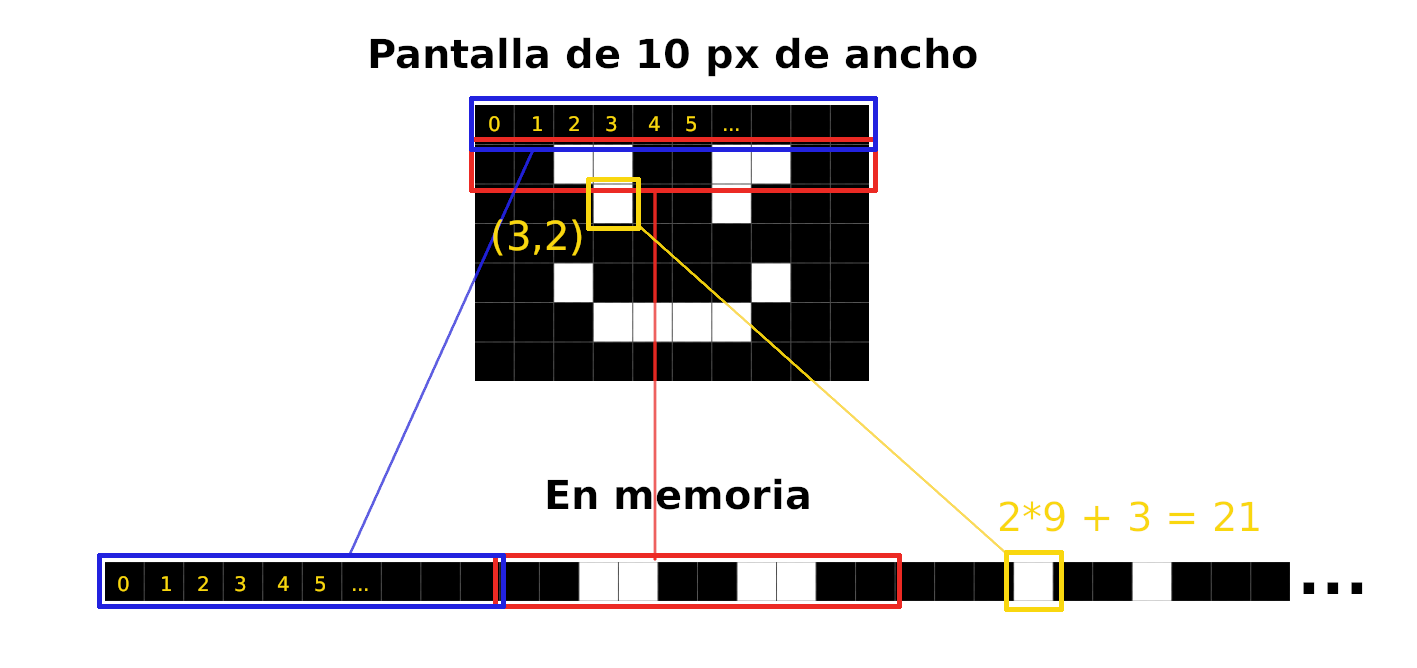
\includegraphics[width=0.8\textwidth]{archivos/screen_vs_memory.png}
  \caption{Comparativa de disposición de pixeles en pantalla y en memoria}
  \label{fig:screen_vs_memory}
\end{figure}

\vspace{0.5cm}

Los pixeles en pantalla están representados por una coordenada (x,y), donde x toma valores en un rango de [0-254] e y en un rango [0-191]. Sin embargo, en memoria esto no es así, pues están representados en 1 dimensión, colocándose una pixel consecutivamente al que le precede. Es por esto que si queremos saber qué posición ocuparía un pixel en memoria, bastaría con realizar el siguiente cálculo:

\vspace{0.5cm}

\begin{equation}
indice = x + ANCHO_{pantalla} * y
\end{equation}

\vspace{0.5cm}

Por ejemplo, para el pixel en coordenadas de pantalla (0,1) siendo el ancho de pantalla 255, el pixel se encontraría en la posición número 255 (0 + 255 * 1), ya que por delante de él hay 255 píxeles que conforman la primera fila de pantalla.

\vspace{0.5cm}

Con esto ya sabríamos en qué posición encontraríamos nuestro pixel, pero esto no es todo, pues nuestro fondo no está en la posición 0x00000000, sino que está donde hemos asignado el banco de memoria de video (0x06200000). Por eso, debemos incrementarle a nuestro resultado dicha posición inicial. Además, también tenemos que tener en cuenta que debemos dividir el resultado entre 2, debido a que los fondos pasan a ser de 8bpp.

\vspace{0.5cm}

El siguiente código muestra una implementación de una función llamada drawPointSub que hace lo explicado anteriormente tomando como parámetros las coordenadas (x,y) de pantalla donde el usuario pulsa. Además de pintar dicho pixel, también pinta los adyacentes formando un círculo como se puede ver en la siguiente figura.

\vspace{0.5cm}

\begin{lstlisting}[caption={Función de dibujado de pixeles dada una entrada de usuario}, label={code:drawPointSub}]

#define SCREEN_START ((u16*)0x06200000) //start of the background video memory
const unsigned int color = 0;  //pixel color

[...]

void Graphics::drawPointSub(int x, int y){

    //calculate the memory address
    int add = x + SCREEN_WIDTH * y;
    add = add/2;

    //draw the pixel
    dmaCopy(&color, SCREEN_START + add , 2);
    
    [...]
}

\end{lstlisting}

\vspace{0.5cm}

\begin{figure}[htbp]
\centering
  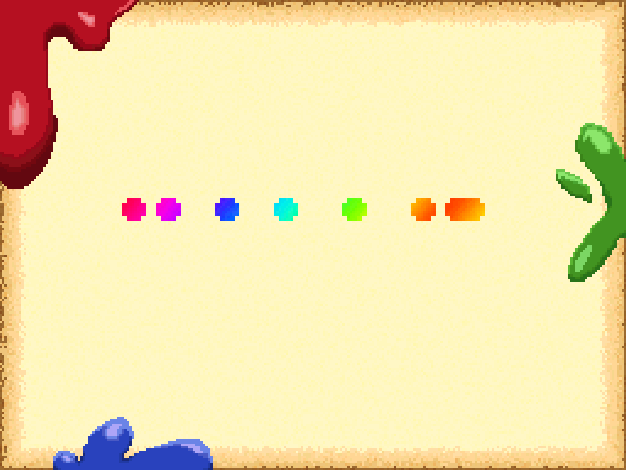
\includegraphics[width=0.5\textwidth]{archivos/sub_draw_no_bresenham.png}
  \caption{Resultado de usar la función drawPointSub para dibujar una línea}
  \label{fig:sub_draw_no_bresenham}
\end{figure}

\vspace{0.5cm}

Esta función era llamada cada vez que el usuario comenzaba a pulsar o mantenía pulsada la pantalla táctil y debería dejar el rastro de éste, sin embargo como vemos en la figura anterior parece que no realiza todo el recorrido, pues dibujé una línea recta. Esto era debido al framerate de la consola, el cual está ajustado a 60 debido a que en cada iteración siempre espera a que se de la interrupción  VBLANK (es decir, cada vez que se termina de dibujar un frame).

\vspace{0.5cm}

Para solucionar esto lo que hice fue, entre frame y frame, en lugar de dibujar un punto concreto dibujar una línea que unía el punto que el usuario estaba pultando actualmente y el que había pulsado en la anterior iteración. Esto lo solventé implementando el algoritmo de Bresenham para dibujado de líneas.

\vspace{0.5cm}

\subsubsection{Algoritmo de Bresenham}

\vspace{0.5cm}

El algoritmo de Bresenham sirve para dibujar en medios discretos gráficos tales como líneas, círcunferencias y otras curvas. A toda la familia de algoritmos se les conoce bajo el mismo nombre ya que parten de la misma idea y pero tienen ligeras modificaciones.

\vspace{0.5cm}

\begin{figure}[htbp]
\centering
  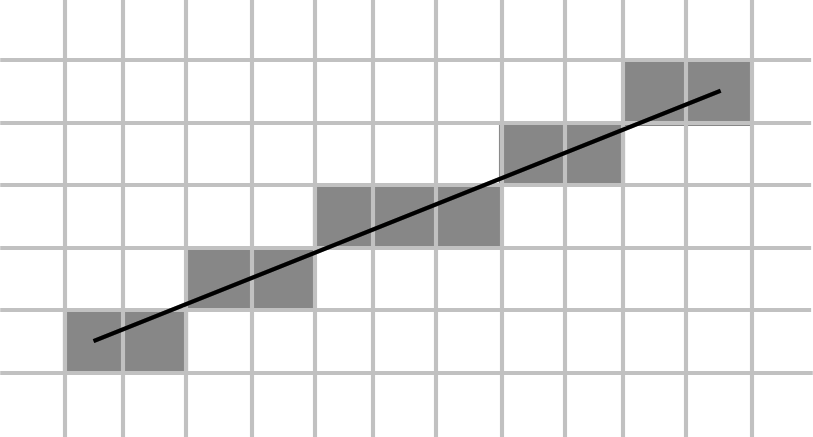
\includegraphics[width=0.5\textwidth]{archivos/bresenham.png}
  \caption{Aplicacion del algoritmo de Bresenham para dibujar líneas en un medio discreto}
    \textbf{Fuente:} \href{https://projectprinter2d.wordpress.com/2015/02/12/point-to-point-with-linear-path-bresenhams-algorithm-implementation/#more-105}{ProjectPrinter2D}
  \label{fig:bresenham}
\end{figure}

\vspace{0.5cm}

El algoritmo de Bresenham para dibujado de lineas se basa en lo siguiente:

\begin{itemize}
 \item  Dados un punto inicial y final de la recta, calculamos las distancias entre los puntos tanto en el eje horizontal como vertical.
 \item Comprobamos qué distancia es mayor, pues la mayor hará que en cada iteración avance siempre en una unidad. Por ejemplo, si una linea es casi o plenamente vertical esta claro que siempre avanzará en una unidad en el eje Y.
 \item En cuanto a la distancia que sea menor, esta a veces avanzará o no avanzará en su eje. Para saber cuándo hacerlo o no, se vale de un valor que llamaremos 'e', que se calcula como la relación entre las distancias por ejes.
 
 \begin{equation}
e = dx / dy
\end{equation}

 \item Cuando este valor es inferior a la unidad, no se avanza y cuando la supera (en cada iteración se acumula), se le resta una unidad y se avanza en ese eje. Esto se puede ver mejor en la siguiente figura.

\end{itemize}

\vspace{0.5cm}

Una vez entendido esto, procedí a implementar el algoritmo. Para ello, dentro de mi clase que maneja todos los gráficos creé una función a la que le pasaría las coordenadas del punto inicial y final y se encarga de llamar a la función que he mencionado antes (drawPointSub) para pintar un punto en la pantalla.

\vspace{0.5cm}

Al principio podemos distinguir dos bloques condicionales, que se encargan de calcular los incrementos tanto en el eje X, como en el Y, en función de la orientación de la línea. Esta puede saberse coprobando si las distancias son negativas. Después, un tercer bloque comprueba la inclinación de esta (si dx >= dx), para ajustar cuál será el incremento que siempre aumentará una unidad en cada iteración. Por último, se hacen los cálculos de los errores para la posterior decisión de incrementar o no el eje de menor distancia.

\vspace{0.5cm}

Una vez calculados estos valores, se inicializan a nuestro punto inicial de la recta unos puntos que llamaremos los 'actuales'. Estos nos servirán de iteradores y se irán actualizando según el algoritmo. Así pues, comenzamos a iterar, siempre dibujando el punto al principio y después realizando los calculos de los errores para ver si incrementamos una unidad en el eje de menor distancia (cuando av sea mayor o igual a 0) y por último actualizamos los puntos actuales. Repetiremos esto hasta que el punto actual coincida con el punto final.

\vspace{0.5cm}

\begin{lstlisting}[caption={Implementación del algoritmo de Bresenham}, label={code:bresenham_algorithm}]

void Graphics::drawLineSub(int x_i, int y_i, int x_f, int y_f){

    int dx = x_f - x_i;
    int dy = y_f - y_i;

    int inc_x_i, inc_x_r, inc_y_i, inc_y_r = 0;

    //Calculamos los desplazamientos en el eje X
    if(dx >= 0){
        inc_x_i = 1;
    }else{
        dx = -dx;
        inc_x_i = -1;
    }

    //Calculamos los desplazamientos en el eje Y
    if(dy >= 0){
        inc_y_i = 1;
    }else{
        dy = -dy;
        inc_y_i = -1;
    }

    //Decidimos cual es el eje de incremento siempre en base a la inclinacion de la recta
    if(dx >= dy){

        inc_x_r = inc_x_i;
        inc_y_r = 0;

    }else{

        inc_x_r = 0;
        inc_y_r = inc_y_i;

        int aux = dx;
        dx = dy;
        dy = aux;
    }

    //Calculamos los errores
    int av_r = 2 * dy;
    int av = av_r - dx;
    int av_i = av - dx;

    //Punto iterador
    int x_act = x_i;
    int y_act = y_i;

    //Bucle
    do{

        //Función de dibujar un punto
        drawPointSub(x_act, y_act);

        if(av >= 0){
        
            //Nos movemos en dos ejes

            //Actualizar el punto
            x_act = x_act + inc_x_i;
            y_act = y_act + inc_y_i;
            //Actualizar el error
            av = av + av_i;

        }else{

            //Nos movemos solo en un eje
            
            //Actualizar el punto
            x_act = x_act + inc_x_r;
            y_act = y_act + inc_y_r;
            //Actualizar el error
            av = av + av_r;

        }

    //Repetir hasta llegar al punto final
    }while(x_act != x_f || y_act != y_f);
}

\end{lstlisting}

\vspace{0.5cm}

Una vez hecho esto, solo falta hacer una pequeña distinción. Llamaremos a esta función siempre que el usuario mantenga pulsado, así pues deberemos tener unas variables que nos permitan saber qué coordenadas se pulsaron en la anterior iteración e ir actualizándolas. Esto nos lleva a un caso, ¿qué pasa si es la primera vez que el usuario pulsa la pantalla? Pues bien, para eso, incicializamos estas variables a un valor negativo y comprobaremos ese valor a la hora de dibujar. Si lo son, dibujaremos un único punto, inicializaremos los puntos y seguiremos y, si no, se aplicará Bresenham. Esto se puede ver en el siguiente código:

\vspace{0.5cm}

\begin{lstlisting}[caption={Llamada a Bresenham}, label={code:bresenham_call}]

[...]

//Si es la primera vez que pulsa la pantalla táctil
if(x_in == -1 && y_in == -1){

    //Dibujamos un punto
    g->drawCircleSub(stylus.px, stylus.py);

//Si no
}else{

    //Nos ahorramos el cálculo si el punto que vamos a dibujar es el mismo que la iteración anterior
    if(x_in != stylus.px || y_in != stylus.py){
    
        //Calcular Bresenham
        g->drawLineSub(x_in, y_in, stylus.px, stylus.py);
    }
}

//Actualizamos el punto
x_in = stylus.px;
y_in = stylus.py;

[...]

\end{lstlisting}

\vspace{0.5cm}

Finalmente, este es el resultado del dibujado de una varias líneas usando dicho algoritmo en la pantalla táctil: 

\vspace{0.5cm}

\begin{figure}[htbp]
\centering
  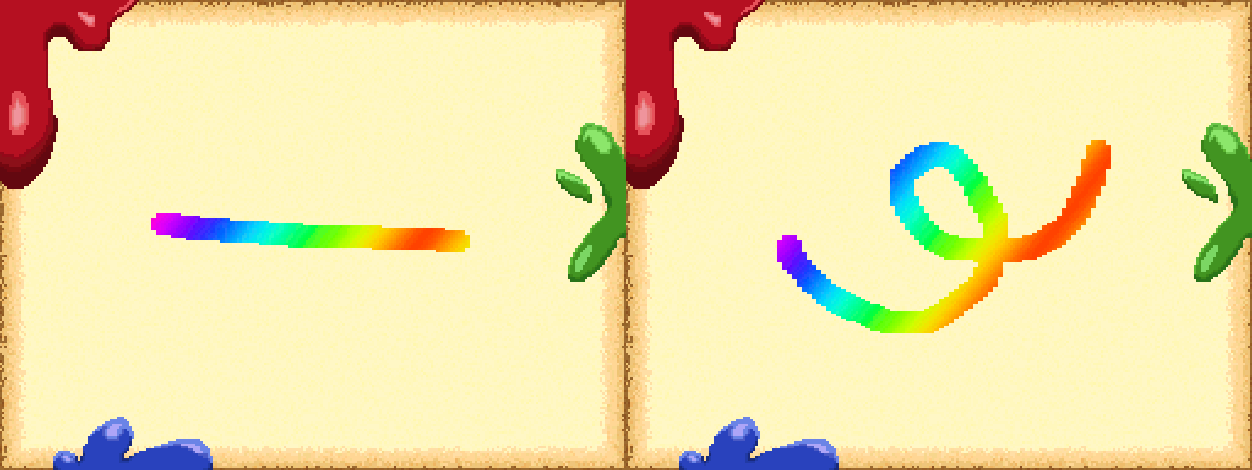
\includegraphics[width=0.7\textwidth]{archivos/sub_draw_bresenham.png}
  \caption{Dibujado en la pantalla táctil usando el algoritmo de Bresenham}
  \label{fig:sub_draw_bresenham}
\end{figure}

\vspace{0.5cm}

Una vez conseguido el dibujado, lo siguiente que hice fue implementar en nuestro proyecto el algoritmo de reconocimiento de gestos desarrollado en la iteración anterior, ya que si bien aún necesitaba algunos retoques, funcionaba bastante mejor que se desarrolló en las primeras iteraciones y ya permitía jugar al usuario.

\vspace{0.5cm}

Para hacer esto, volví a recurrir al diseño de clases del proyecto, pensando cómo podría incluir el uso de este algoritmo de una forma abstraída y limpia. Entonces mi solución fué crear una clase llamada PatternManager, que fuese accesible desde Level. Esta clase contendría tanto los patrones ideales como el patrón usuario, es decir, unas estructuras de datos (arrays y vectores) y unos métodos para trabajar con ellos, como són los siguientes:

\vspace{0.5cm}

\begin{itemize}
 \item checkPattern(): Toma como parámetro el patrón ideal con el que quiere comparar el del usuario y realiza el algoritmo descrito en la anterior iteración, devolviendo un número decimal que representa el error total entre ambos patrones.
 \item insertPoint(): Pasandole como parámetro la coordenada x e y del punto de pantalla que el usuario ha pulsado, inserta un nuevo elemento en el array de puntos que conforman el trazo del usuario.
 \item clearPattern(): Borra todos los elementos del array de puntos que conforman el trazo del usuario.
\end{itemize}

A continuación se muestra un esquema de diagrama de clases que muestra la relación de las clases PatternManager y Level:

\vspace{0.5cm}

\begin{figure}[htbp]
\centering
  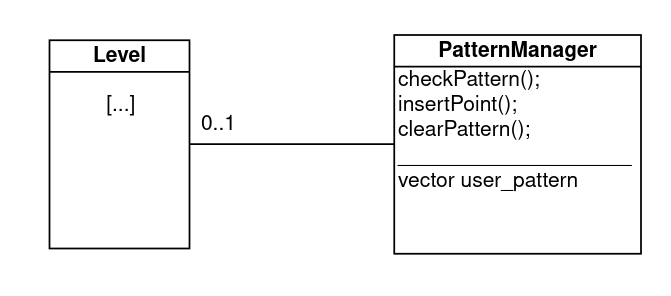
\includegraphics[width=0.5\textwidth]{archivos/diagram_patternmanager.png}
  \caption{Diagrama de la relación entre las clases Level y PatternManager}
  \label{fig:diagram_patternmanager}
\end{figure}

\vspace{0.5cm}

Por último, lo que implementé durante esta iteración fue una mejora en los enemigos. Para que fuesen similares a nuestro referente, Magic Cat Academy, jugué varias veces a éste y me percaté de que más o menos, los enemigos siempre salían por las mismas zonas, las cuales muestro en la siguiente figura:

\vspace{0.5cm}

\begin{figure}[htbp]
\centering
  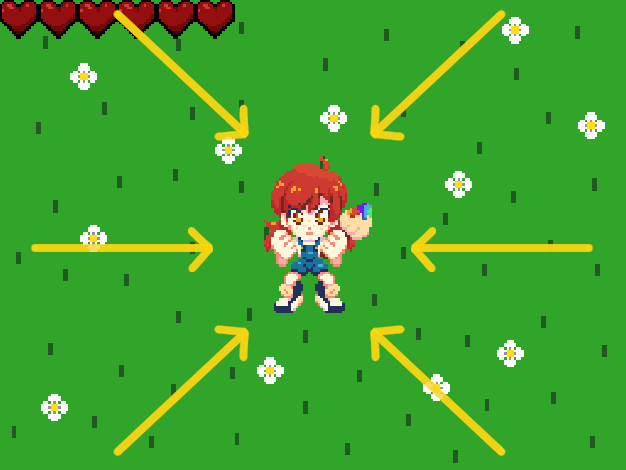
\includegraphics[width=0.5\textwidth]{archivos/spawn_enemies_position.png}
  \caption{Definición visual de las posiciones iniciales y caminos de los enemigos}
  \label{fig:spawn_enemies_position}
\end{figure}

\vspace{0.5cm}

Así pues, lo que hice principalmente fue definir 6 posiciones fijas y al crear un enemigo, se le asigna una de estas posiciones. No obstante, como ahora el update de cada enemigo sería distinto (unos se mueven recto, otros inclinados, etc), tuve que definir dos nuevas variables que se iniciarían justo al definir esta posición del enemigo. Estas variables son inc\_x e inc\_y, las cuales definen el camino que seguirá el enemigo.

\vspace{0.5cm}

Ahora bien, lo último que quedaba era asegurarse de que todos los enemigos que saliesen de la parte izquierda de la pantalla, tuviesen el sprite invertido horizontalmente, para que mirasen hacia la dirección en la que avanzan. Esto se puede hacer fácilmente gracias a libnds y la estructura SpriteEntry, de la cual ya hemos hablado, tan solo debemos asignar la propiedad hFlip a verdadero, sin embargo, nos esto nos pone un impedimento, y es que libnds nos dice que para poder invertir un sprite es necesario que una de sus otras propiedades, isRotateScale sea falso. Esto quiere decir que no podemos aplicar sobre el sprite transformaciones afines de escalado y rotado, con lo cual debemos tenerlo en cuenta.

\vspace{0.5cm}

Lo último que hice fue asignar bien las prioridades de los sprites para que algunos se viesen por encima de otros, de la siguiente manera:

\vspace{0.5cm}

\begin{itemize}
 \item Prioridad 0: Los sprites de la vida del jugador, siempre por encima de todo.
 \item Prioridad 1: Los enemigos que vienen desde la línea inferior
 \item Prioridad 2: El jugador.
 \item Prioridad 3: Los enemigos que vienen desde la línea central o la superior.
\end{itemize}

\vspace{0.5cm}

Y este fue el resultado de los enemigos con el nuevo cambio en funcionamiento:

\vspace{0.5cm}

\begin{figure}[htbp]
\centering
  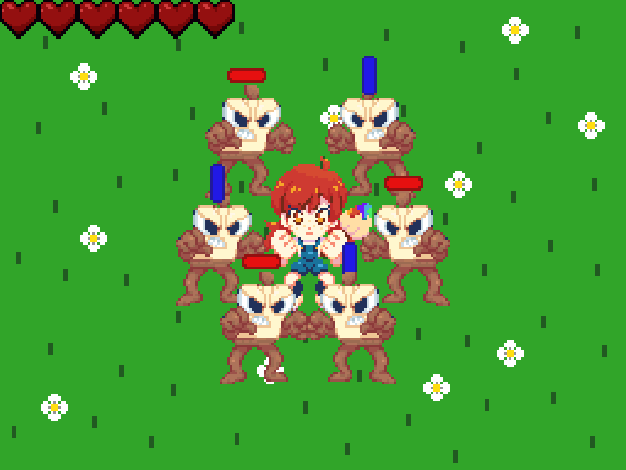
\includegraphics[width=0.5\textwidth]{archivos/spawn_enemies_position_2.png}
  \caption{Resultado de esta implementación}
  \label{fig:spawn_enemies_position_2}
\end{figure}

\vspace{0.1cm}

\subsection{Iteración 5 - Retoques al algoritmo de reconocimiento de gestos y animaciones}

Durante esta quinta iteración planifiqué centrarme en varios aspectos relativos al algoritmo de reconocimiento de gestos para así poder dejarlo completamente terminado.

\vspace{0.5cm}

Si bien el algoritmo ya estaba implementado en el juego y sus resultados eran buenos, aún quedaban algunos aspectos por revisar y perfeccionar, pues probándolo me di cuenta de dos problemas que tenía. El primero de ellos es, que según la forma de realizar el cálculo de la desviación entre los puntos de los trazos, el trazo dibujado por el usuario debía tener el mismo sentido que el que nosotros tomábamos por ideal. Tanto el trazo del usuario como el ideal están almacenados en estructuras de tipo array, donde los puntos son accesibles gracias a un índice que va de 0 hasta el tamaño total de la estructura. Pues bien, el algoritmo al comenzar a iterar los puntos del trazo del usuario lo hace siguiendo ese orden, desde 0 hasta el tamaño máximo, calculando las desviaciones entre pares de puntos que comparten el mismo índice, es decir, el punto 0 con el 0, el 1 con el 1, etc.

\vspace{0.5cm}

Esto podemos visualizarlo mejor gracias a la siguiente figura. Supongamos un trazo ideal que sea una línea horizontal de 3 puntos: p1(0,0), p2(1,0) y p3(2,0), por simplificación. En nuestro código, hemos decidido que se almacenarían en ese mismo orden, correspondiendo el índice 0 a p1, el 1 a p2 y el 2 a p3. Ahora el usuario, al ver que para poder jugar debe dibujar una línea horizontal la dibuja siguiendo el orden inverso por preferencia suya, es decir, que su línea almacenada en nuestro programa sería p1(2,0) en el índice 0, p2(1,0) en el 1 y p3(0,0) en el 2. Si realizamos el cálculo en el orden de los índices la desviación total que nos da es aproximadamente 2,82, lo cual es erróneo pues ambas líneas son exactamente iguales y la desviación debería ser nula. En la imágen está representado mediante flechas rojas los cálculos que actualmente realiza el algoritmo y que son erróneos y, en verde los que debería realizar por lógica.

\vspace{0.5cm}

\begin{figure}[htbp]
\centering
  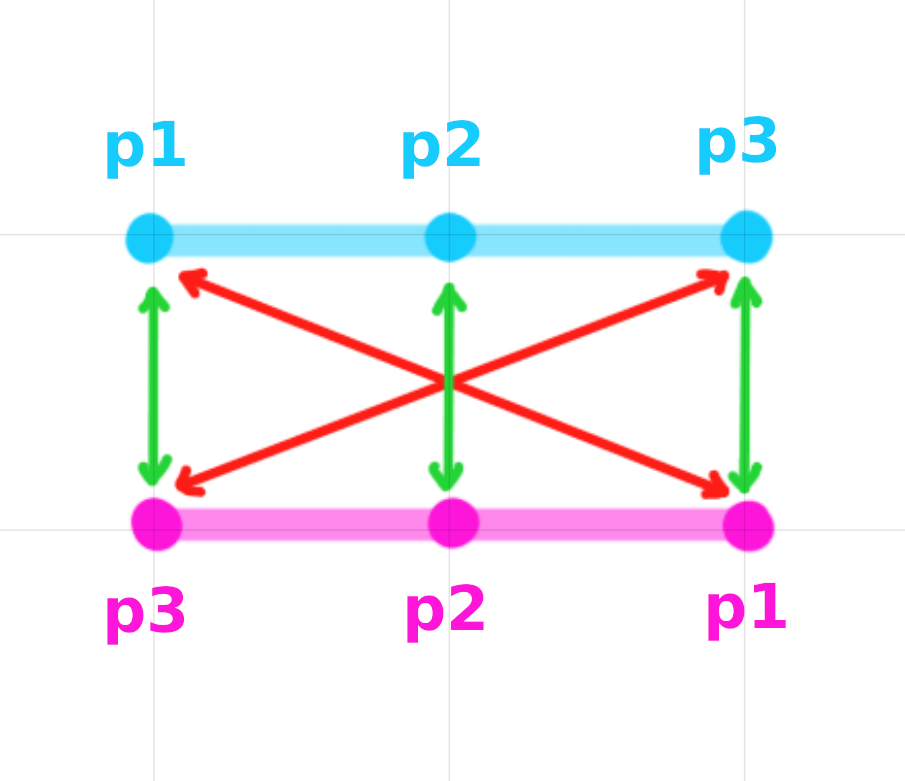
\includegraphics[width=0.5\textwidth]{archivos/findnearest.png}
  \caption{Ejemplo visual del cálculo de la desviación entre los puntos de dos trazos}
  \label{fig:findnearest}
\end{figure}

\vspace{0.5cm}

Si nos fijamos bien en los algoritmos que hemos estudiado previamente como PAlib y Graffiti, vemos que estos sí tienen en cuenta el sentido de dibujado del trazo y diferencian, por ejemplo, en PAlib las líneas que han sido dibujadas de izquierda a derecha y viceversa representan distintos caracteres dado que sus ángulos son distintos. Además, por lo general la gran mayoría de trazos que representan letras se dibujan de izquierda a derecha. No ibstante, nuestro referente en cuanto a mecánicas y jugabilidad, Magic Cat Academy, ignora el sentido del trazo y se centra en que la forma en general sea la correcta. Esto me parece más intuitivo, pues al tratarse de un juego al que pueden jugar tanto personas zurdas, diestras, o incluso alguna persona con discapacidad motora, obligarle a realizar el trazo en un sentido concreto puede afectar negativamente a su experiencia de usuario. Así pues, decidí tratar este problema y resolverlo haciendo que el cálculo de la desviación se realizase entre dos puntos cuya distancia sea mínima.

\vspace{0.5cm}

Para hacer el cálculo entre los puntos de menor distancia hice una función llamada findNearest que toma como argumentos unas coordenadas x e y, y el trazo ideal del cual se quiere buscar el más cercano. Así pues, cada vez que desde nuestro algoritmo principal estemos procesando un punto del trazo del usuario se llamará a esta función para que nos devuelva el punto del trazo ideal de menor distancia a este.

\vspace{0.5cm}

\begin{lstlisting}[caption={Búsqueda del punto más cercano con la función findNearest}, label={code:findNearest}]
int PatternManager::findNearest(int x, int y, const Vector2D shape[]){

	float dist = FLT_MAX;
	int nearest = -1;

	for(int i = 0; i<ANCHOR_POINTS; i++){

		Vector2D pos = shape[i];

        //calculamos la distancia
		float dist_act = sqrt(pow((pos.getX()-x),2)+pow(pos.getY()-y,2));

		if(dist_act < dist){ // actualizamos el punto de menor distancia
			nearest = i;
			dist = dist_act;
		}
	}

	return nearest;

}
\end{lstlisting}

\vspace{0.5cm}

El código anterior muestra el funcionamiento de la función findNearest. Lo que hace básicamente es comenzar a recorrer el array del trazo ideal calculando la distancia entre el punto sobre el que está iterando y el punto pasado por parámetro. Si esta distancia es menor, se actualizan tanto una variable que guarda dicho valor de la distancia para ser comparado con los demás y el índice de ese punto, que será lo que la función da como resultado.

\vspace{0.5cm}

El cálculo de la distancia puede resultar algo engorroso de ver tal y como está escrito en el código, por ello se muestra en la siguiente fórmula:

\vspace{0.5cm}

 \begin{equation}
d(AB) = \sqrt{(x_b-x_a)^{2}+(y_b-y_a)^{2}}
\end{equation}

\vspace{0.5cm}

Las funciones pow() y sqrt() de la librería de sistema math.h nos proporcionan el cálculo de la potencia y raíz cuadrada respectivamente.

\vspace{0.5cm}

Con esto y tendríamos solucionado este problema, no obstante al haber hecho una modificación tan importante como añadir un bucle más al algoritmo hemos de tener en cuenta que ahora su tiempo de ejecución ha aumentado, pues ha pasado de ser un simple bucle (complejidad lineal) a ser un bucle anindado (complejidad cuadrática). Esto puede ser un problema si decidimos aumentar el número de puntos de muestra de cada patrón o incluso si añadimos muchos más patrones distintos. Recordemos que este cálculo es algo que se debe realizar con la mayor rapidez posible, pues de lo contrario podría provocar tirones en el juego y repercutiría negativamente en la experiencia del usuario. No obstante, como de momento tenemos pocos puntos de muestra y pocos patrones vamos a centrarnos primero en resolver el siguiente problema.

\vspace{0.5cm}

En cuanto al segundo problema, este se debe a la forma en la que desplazamos el trazo del usuario hacia el trazo ideal para realizar posteriormente el cálculo de la desviación. Como ya hemos comentado, elegíamos el punto inicial de ambos trazos, calculábamos el desplazamiento y después cuando iterabamos sobre los puntos del trazo del usuario los íbamos desplazando. El hecho de usar el punto inicial tenía sentido si, nuevamente, todos los trazos tuvieran que ser hechos con el mismo sentido que los ideales. Sin embargo, al no tener en cuenta esto y dejando el algoritmo tal y como estaba, el trazo del usuario se desplazaria de tal forma que el cálculo de la desviación podría dar unos valores incorrectos. Esto se puede ver mejor en la siguiente figura.

\vspace{0.5cm}

\begin{figure}[htbp]
\centering
  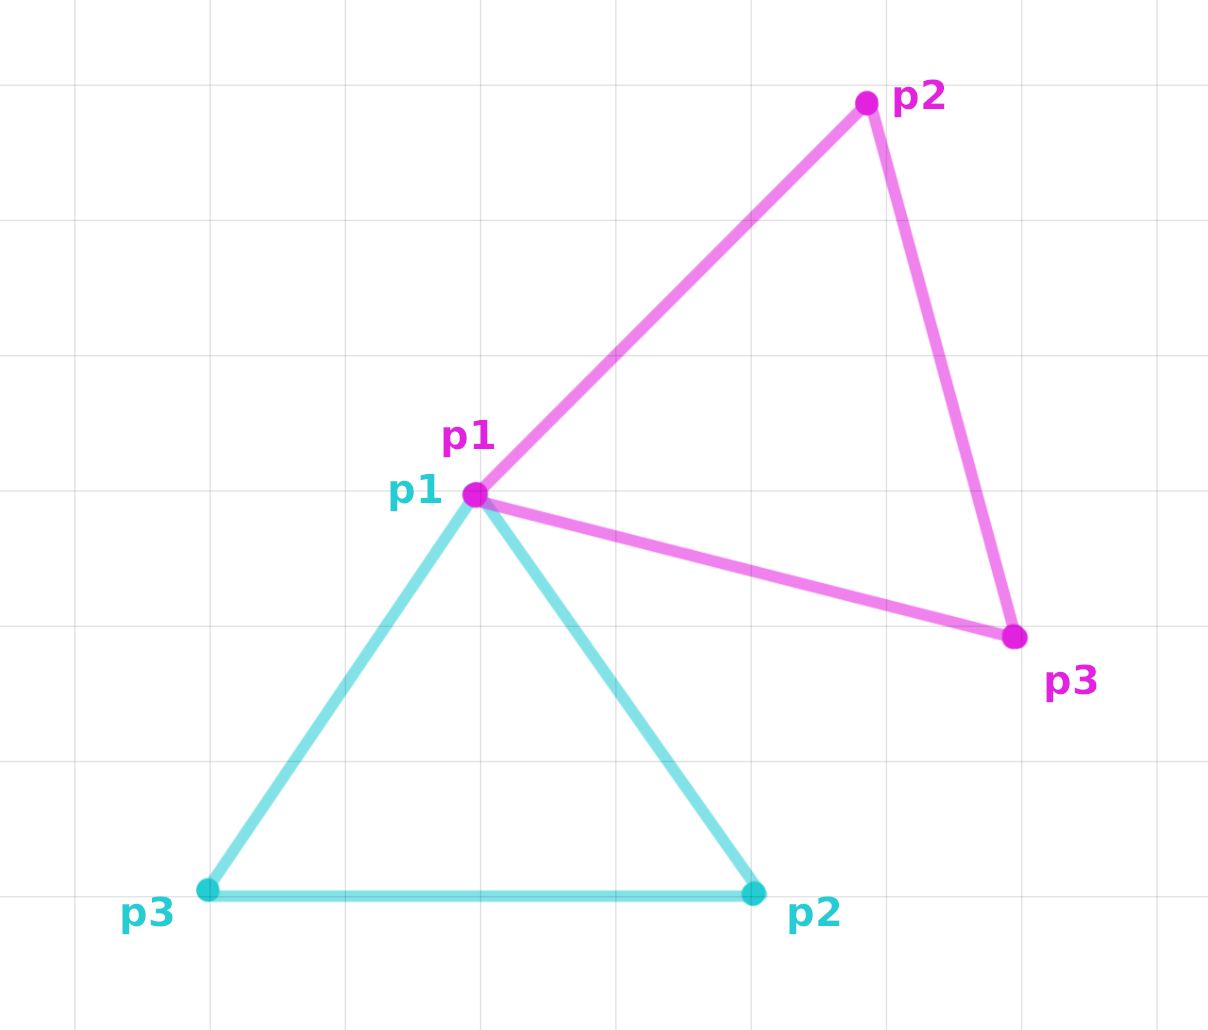
\includegraphics[width=0.5\textwidth]{archivos/not_center_of_mass.png}
  \caption{Desplazamiento erróneo del trazo del usuario (rosa) con respecto al trazo ideal (azul)}
  \label{fig:not_center_of_mass}
\end{figure}


\vspace{0.5cm}

Como solución a este problema, debía desplazar todo el trazo a un punto que representase el centro del mismo y que pueda ser calculado para cualquier nube de puntos, este es el centro de masas.

\vspace{0.5cm}

La fórmula del cálculo del centro de masas es la siguiente, donde r representa el vector de posición (x,y) del punto, m su masa y M el valor total de la masa del sistema.

\vspace{0.5cm}

 \begin{equation}
r_{cm} = \frac{\sum _i m_ir_i}{\sum _i m_i} = \frac{1}{M} \sum_{i} m_ir_i
\end{equation}

\vspace{0.5cm}

 No obstante, si bien el centro de masas es un concepto con el que podemos trabajar en ámbitos donde los puntos u objetos de un sistema posean un peso, en nuestro caso podemos asumir que todos nuestros puntos tienen el mismo peso o importancia, en este caso la unidad. Así pues, la fórmula quedaría de la siguiente manera:
 
 \vspace{0.5cm}
 
 \begin{equation}
r_{cm} =\frac{1}{N} \sum_{i = 0}^{N} r_i = \frac{r_0+r_1+r_2+...+r_n}{N} 
\end{equation}
 
 \vspace{0.5cm}
 
 Una vez entendido esto, para implementarlo en el código creé una función llamada calculateCenterOfMass() que recorre el vector que conforma el trazo del usuario, selecciona los puntos de muestra y los acumula para calcular así el centro de masas y almacenar sus coordenadas luego en dos variables, x\_cm e y\_cm.
 
 \begin{lstlisting}[caption={Cálculo del centro de masas con la función calculateCenterOfMass()}, label={code:calculateCenterOfMass}]
void PatternManager::calculateCenterOfMass(){

	int sum_x = 0;
	int sum_y = 0;

	x_cm = 0;
	y_cm = 0;

	//iterador sobre los puntos de muestra
	float inc = (user_pattern.size()-1)/(ANCHOR_POINTS-1);
	float j = 0.0;

	for(int i=0;i<ANCHOR_POINTS;i++){
		if(user_pattern[i]){

			Vector2D* pos = user_pattern[j];

			sum_x = pos->getX() + sum_x; //acumulamos la coordenada X
			sum_y = pos->getY() + sum_y; //acumulamos la coordenada Y

		}

		if(i == ANCHOR_POINTS-1){
			j = user_pattern.size()-1;
		}else{
			j = j + inc;
		}
	}

	//dividimos entre el total de puntos
	x_cm = sum_x/ANCHOR_POINTS;
	y_cm = sum_y/ANCHOR_POINTS;

}
\end{lstlisting}

 \vspace{0.5cm}

A pesar de haber añadido nuevamente una tarea más al algoritmo esto no supone un gran problema como puede ser el anterior a nivel de coste, pues este cálculo se va a realizar una única vez cada vez que el usuario dibuje un patrón ya que el centro de masas es el mismo para realizar los cálculos con todos los patrones ideales que tengamos.

 \vspace{0.5cm}

Además, los centros de masas de los patrones ideales los almacené en un array y así ir usando los que me convenga. Por ejemplo, el usuario dibuja un trazo, seguidamente calculo el centro de masas de ese trazo, paso a realizar el cálculo de desviaciones entre ambos y en ese proceso uso ese array para obtener el centro de masas del patrón ideal en concreto.

 \vspace{0.5cm}
 
 Por último lo que realicé para ver que efectivamente estaba calculando bien el centro de masas fue utilizar la función drawCircleSub() para dibujar en pantalla dicho centro, siendo este el resultado:
 
\vspace{0.5cm} 
 
 Como se puede ver, parece que el centro está algo desplazado, pero esto es normal pues hemos dibujado dos patrones que se tratan de figuras cerradas, haciendo que dos de sus puntos, en concreto el inicial y final, sean prácticamente el mismo y por tanto haciendo que este centro se desvie hacia donde se encuentran estos. Esto no es gran problema, pues este desvío será así para todas las figuras y no afectará negativamente al cálculo.
 
  \vspace{0.5cm}
  
\begin{figure}[htbp]
\centering
  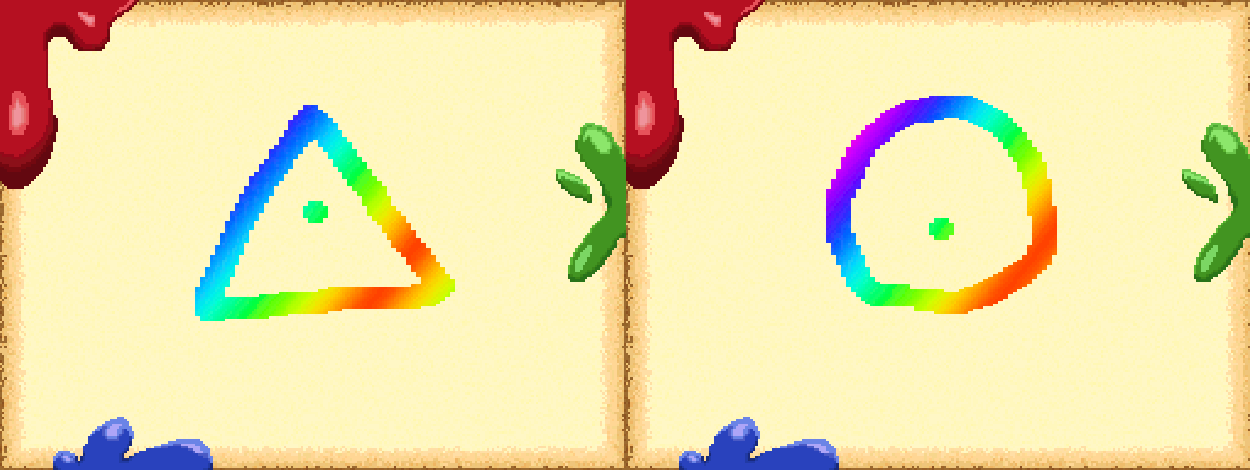
\includegraphics[width=0.7\textwidth]{archivos/yes_center_of_mass.png}
  \caption{Dibujado de un trazo y señalización de su centro de masas}
  \label{fig:yes_center_of_mass}
\end{figure}
  
\vspace{0.5cm}
  
  Lo último que realicé durante esta iteración fue comenzar a darle algunos toques visuales al juego, comenzando por las animaciones de los sprites.
  
   \vspace{0.5cm}
  
  Comencé por la animación de la protagonista que, a pesar de encontrarse en el centro de la pantalla y no moverse, decidí darle un toque más de vida y hacerle una animación para que pareciese que está preparada para luchar.
  
   \vspace{0.5cm}
  
  Usando el sprite inicial, en GIMP separé por capas los distintos elementos que quería mover, como la cabeza, cuerpo, manos y pies, y los fui colocando y creando los diferentes frames. El resultado fue el siguiente:
  
   \vspace{0.5cm}
  
\begin{figure}[htbp]
\centering
  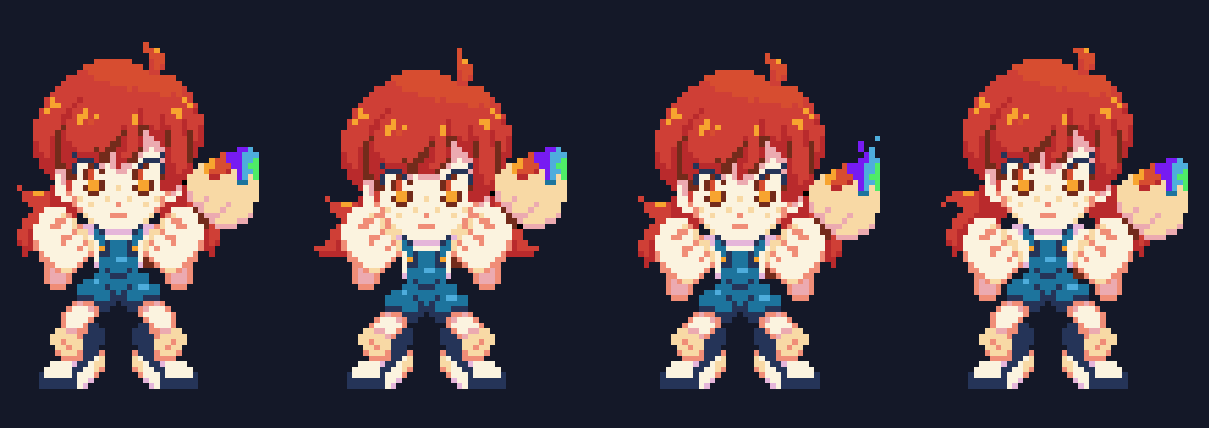
\includegraphics[width=0.7\textwidth]{archivos/player_animation.png}
  \caption{Frames de la animación del jugador}
  \label{fig:player_animation}
\end{figure}

\clearpage
  
  Para implementar la animación en el juego símplemente cargué todos los frames consecutivamente. Después, en la clase Player añadí una variable de tipo entero llamada animation\_clock, que es inicializada a un valor concreto. En cada iteración este valor se decrementará en una unidad y cuando llegue a 0 llamaremos a una función de la fachada para que se encargue de cambiar el sprite al siguiente frame.
  
   \vspace{0.5cm}
  
   \begin{lstlisting}[caption={Animación del sprite del jugador}, label={code:animacionplayer}]
void Player::update(){

	if(animation_clock == 0){
		animation_clock = 8;
		Graphics::Instance()->animatePlayer(getOAMid());
	}else{
		animation_clock--;
	}
}

[...]

void Graphics::animatePlayer(int id){
    SpriteEntry* sprite = &oam->oamBuffer[id];

    if(sprite->gfxIndex < 320){
        sprite->gfxIndex+= 64;
    }else{
        sprite->gfxIndex = 64;
    }

    updateOAM();
}
\end{lstlisting}

   \vspace{0.5cm}
  
Ahora bien, si estamos hablando de animaciones, ¿por qué no he usado un reloj para saber cuánto tiempo ha transcurrido entre ciclos? Pues porque después de valorarlo, no me parecía necesario. Nuestro juego va a ser un programa que se ejecute siempre en el mismo procesador, en el ARM9 y ARM7 de la NDS, es por ello que siempre nos vamos a asegurar de que en todas las consolas nuestro programa funciona exactamente igual, pues sus componentes son los mismos. SIn embargo hay una excepción a esto: la NDSi.

 \vspace{0.5cm}

Como ya hemos comentado anteriormente, la NDSi fue un modelo actualizado de la familia NDS que no solo añadía características innovadoras como las dos cámaras, sino que también posee mejoras a nivel de hardware. El procesador ARM9 es más veloz que el que posee la NDS original, mientras que el ARM7 se mantiene igual. Pero si esto es así, ¿significaría que nuestro juego funcionará más rápido en la NDSi? Pues no, porque Nintendo a la hora de desarrollar esta consola creó el llamado "DSi mode", que es una característica que porta el cartucho del programa y que le dice a la consola si dicho programa puede usar todos los nuevos recursos de DSi. Por supuesto, los juegos desarrollados hasta la fecha de salida de la NDSi no tenían este modo, así que a efectos prácticos funcionaban igual en ambas consolas. En cuanto a nuestra parte, lo único que nosotros podemos usar para poder probar nuestro juego en una NDS real son los cartuchos flash, y el único que tiene soporte para este modo se trata de CycloDSi Evolution, el cual fue inhabilitado por Nintendo mediante una actualización al software de DSi debido a temas de piratería.

 \vspace{0.5cm}

En resumen, nuestro juego va a funcionar siempre con la misma frecuencia de procesador, por ello no tenemos que preocuparnos de que las animaciones puedan verse afectadas al no usar un reloj.

\vspace{1cm}

\subsection{Iteración 6 - Mejoras visuales, corrección de niveles y mejora del producto final}

Al tratarse esta de la penúltima iteración, me centré en acabar algunos aspectos de feedback visual y jugabilidad, así como también de producto.

 \vspace{0.5cm}

En primer lugar, siguiendo donde dejé la iteración pasada las animaciones, quise incorporar las animaciones de los enemigos al moverse. 

 \vspace{0.5cm}

Al igual que hice con el jugador, primero abrí en GIMP el sprite del enemigo para que me sirviese de base para crear los frames de la animación, aunque en este caso al tratarse de un movimiento más complejo sí que tuve que ir deteniendome en cada frame a dibujar sus piernas en cada posición. El resultado fue el siguiente:

 \vspace{0.5cm}

\begin{figure}[htbp]
\centering
  
\includegraphics[width=0.7\textwidth]{archivos/enemy_animation.png}
  \caption{Frames de la animación del enemigo}
  \label{fig:enemy_animation}
\end{figure}

 \vspace{0.5cm}

Seguidamente, para incorporarlo al juego usé nuevamente un contador a modo de temporizador, sin embargo la diferencia de éste es que solo se iba a actualizar si el enemigo se estaba moviendo, es decir, que aún no hubiese alcanzado al jugador.

 \vspace{0.5cm}

   \begin{lstlisting}[caption={Animación del sprite del enemigo al moverse}, label={code:animacionenemy}]
void Enemy::update(){

	if(!checkCollision()){

		x = x + inc_x;
		y = y + inc_y;

		//actualizamos la animación al igual que haciamos con el jugador
		if(animation_clock == 0){
			animation_clock = 8;
			Graphics::Instance()->animateEnemyRun(getOAMid());
		}else{
			animation_clock--;
		}

	}else{
		attack();
		//Como ha llegado hasta el jugador, le asignamos el sprite de estar parado
		Graphics::Instance()->resetEnemySprite(getOAMid());
	}

}

[...]

void Graphics::animateEnemyRun(int id){
    SpriteEntry* sprite = &oam->oamBuffer[id];

    if(sprite->gfxIndex < 256){
        sprite->gfxIndex+= 64;
    }else{
        sprite->gfxIndex = 64;
    }
}
}
\end{lstlisting}

 \vspace{0.5cm}

Después de incorporar esto al juego, cambié el fondo del nivel al que sería el definitivo. Para ello, como siempre primero realicé un boceto previamente y una vez estaba satisfecha con la idea, lo realicé en pixelart con la herramienta GIMP. Una vez terminado, lo incluí al juego simplemente sustituyendo el archivo por el que previamente estaba usando como fondo de nivel.

\clearpage

\begin{figure}[htbp]
\centering
  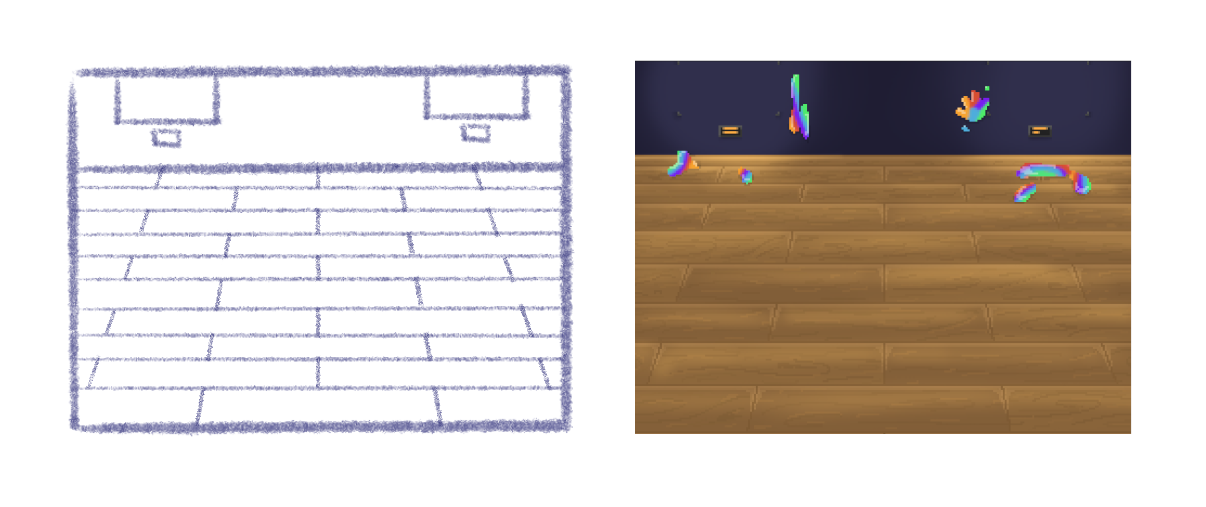
\includegraphics[width=0.8\textwidth]{archivos/level_bg.png}
  \caption{Boceto del fondo de nivel y versión acabada}
  \label{fig:level:bg}
\end{figure}

 \vspace{0.5cm}

Una vez terminado esto, la siguiente tarea que realicé fue una que  contribuiría al que el juego se empezase a ver como un producto más acabado. La NDS, al tener un firmware que se ejecuta al encenderla nos deja ver algunas características de los juegos que tiene insertados en sus ranuras de NDS y GBA. Estas características son el título del juego y un pequeño icono.

 \vspace{0.5cm}

Hasta ahora, al estar usando el Makefile que venía en los ejemplos de devkitPro nos asignaba un nombre y un icono por defecto como podemos ver en la siguiente figura.

 \vspace{0.5cm}

\begin{figure}[htbp]
\centering
  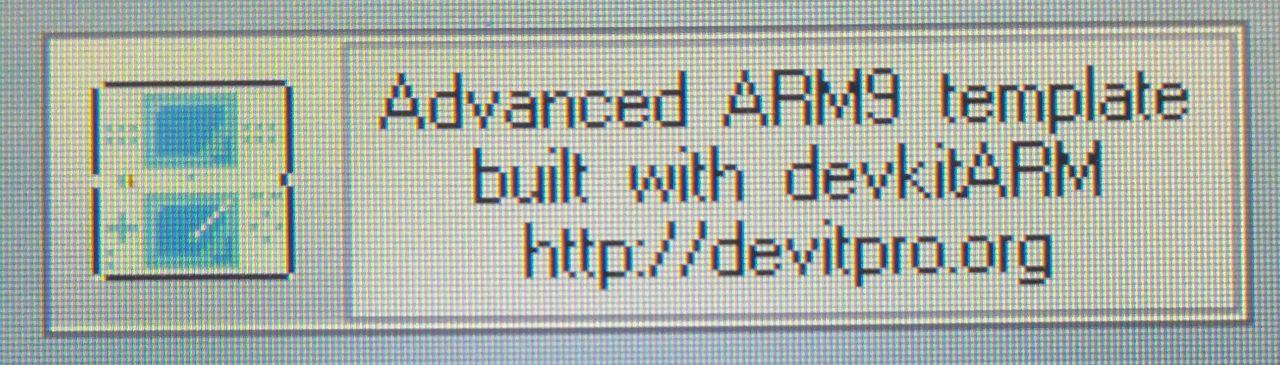
\includegraphics[width=0.7\textwidth]{archivos/icon_default.jpg}
  \caption{Icono y título por defecto de un proyecto de NDS que use devkitARM}
  \label{fig:icon_default}
\end{figure}

 \vspace{0.5cm}

No obstante, dicho archivo ya va preparado para que puedas cambiarlos sin tener que indagar mucho en el código. En concreto, tenemos que buscar las variables con nombre GAME\_TITLE y GAME\_SUBTITLE1 para cambiar el título y la variable ICON para cambiar el icono de la aplicación. A esta última debemos asignarle la ruta a un archivo de 32x32 píxeles y formato BMP de 16 colores (siendo el primer color el transparente). Así pues creé un icono de esas características nuevamente en GIMP y lo incluí al proyecto. El siguiente código muestra los cambios que realicé al Makefile para añadir estas nuevas propiedades al proyecto.

 \vspace{0.5cm}

   \begin{lstlisting}[caption={Cambios en el Makefile para establecer el título y el icono}, label={code:gamenamemakefile}]
[...]

ICON     := ../ icon.bmp

[...]

# These set the information text in the nds file
GAME_TITLE     := Touch & Brush
GAME_SUBTITLE1 := Carla Macia Diez
GAME_SUBTITLE2 := 

[...]

\end{lstlisting}

 \vspace{0.5cm}

Al probar este cambio en la consola real, vi que el título se había cambiado sin problema, sin embargo la imágen parecía tener los colores muy diferentes, aunque la forma se podía visualizar.

 \vspace{0.5cm}

\begin{figure}[htbp]
\centering
  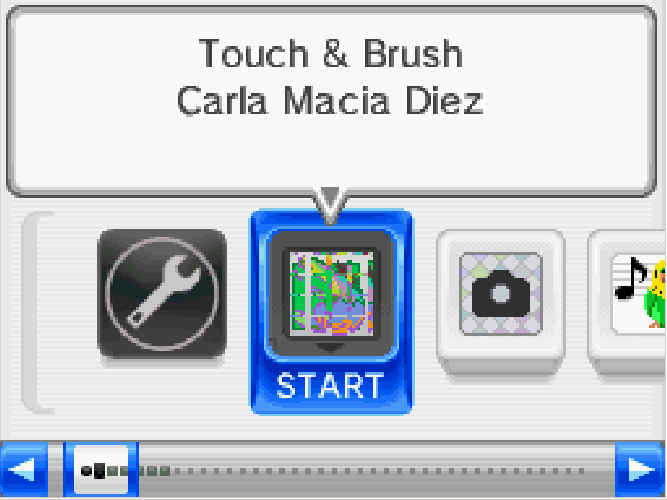
\includegraphics[width=0.7\textwidth]{archivos/icon_corrupted.png}
  \caption{Erronea visualización del icono de la aplicación (firmware de NDSi emulado en no\$gba)}
  \label{fig:icon_corrupted}
\end{figure}

 \vspace{0.5cm}

Pensé que esto podía ser un problema de mi imágen, así que por asegurarme la reemplacé por la que usa por defecto y el problema seguía persistiendo. Fue entonces cuando pensé que a la hora de compilar, debía estar haciendole algun cambio a la imágen original para que se viese de esa forma. Me fijé en la terminal a la hora de compilar el proyecto, y vi que aparecía un mensaje como el siguiente:

\clearpage

\begin{figure}[htbp]
\centering
  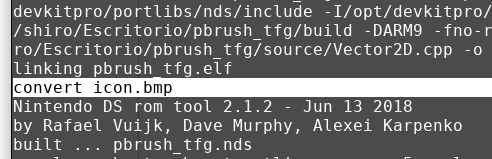
\includegraphics[width=0.8\textwidth]{archivos/convert_grf.png}
  \caption{Mensaje de conversión del Makefile}
  \label{fig:convert_grf}
\end{figure}

 \vspace{0.5cm}

Esto ya me parecía raro, pues si la propia documentación te explica que el formato debe ser BMP, ¿por qué lo convierte? Así pues busqué en qué parte del Makefile realizaba esa conversión y encontré lo siguiente:

 \vspace{0.5cm}

   \begin{lstlisting}[caption={Conversión del archivo BMP a GRF en el Makefile}, label={code:bmptogrfmakefile}]

#---------------------------------------------------------------------------------
# Convert non-GRF game icon to GRF if needed
#---------------------------------------------------------------------------------
$(GAME_ICON): $(notdir $(ICON))
##---------------------------------------------------------------------------------
	@echo convert $(notdir $<)
	@grit $< -g -gt -gB4 -gT FF00FF -m! -p -pe 16 -fh! -ftr

-include $(DEPSDIR)/*.d

\end{lstlisting}

 \vspace{0.5cm}

Fue entonces cuando se me ocurrió probar a quitar dicha conversión a GRF por ver si el formato de mi archivo era válido, así que comenté esa parte del código y asigné directamente a la variable GAME\_ICON la ruta a mi archivo. Y en efecto, ahí estaba el problema, ahora el icono se veía sin ningún problema.

 \vspace{0.5cm}

\begin{figure}[htbp]
\centering
  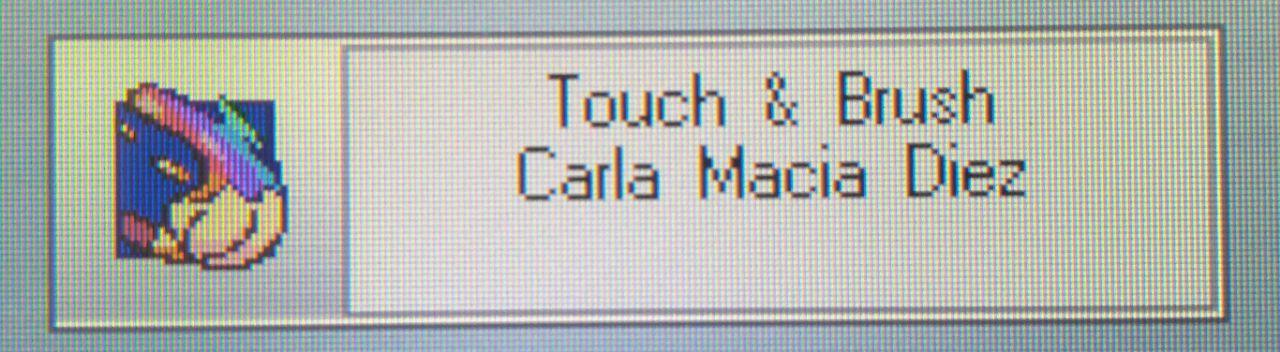
\includegraphics[width=0.7\textwidth]{archivos/icon_good.jpg}
  \caption{Frames de la animación del enemigo}
  \label{fig:icon_good}
\end{figure}

 \vspace{0.5cm}

Ya finalizada esta tarea, seguí con otro aspecto visual de la pantalla del menú principal. Quería asignarle los fondos definitivos tal y como se especifican en el apartado de Pantallas del Diseño del juego.

 \vspace{0.5cm}

Comencé por la pantalla inferior, donde quería colocar un fondo con un mensaje de "Tocar la pantalla para jugar". Además, quería que este siguiese la estética también definidos en el apartado mencionado del Diseño del juego, por ello quise que este texto fuese cambiando de color pasando por todos los tonos, dando así un aspecto de arcoiris.

 \vspace{0.5cm}

Para lograr esto, primero hice el fondo base con el texto sobre él y dicho texto le aseigné un color llamativo como es el fucsia. Después, incluí el fondo al proyecto e hice que se dibujase también cuando se carga el menú principal en la funcion loadMenu() de la clase Graphics. Una vez hice esto, usando la herramienta de depurado visual de la gráficos de no\$gba, vi en qué posicion o posiciones de la memoria de paletas se encontraba este color. 

 \vspace{0.5cm}

\begin{figure}[htbp]
\centering
  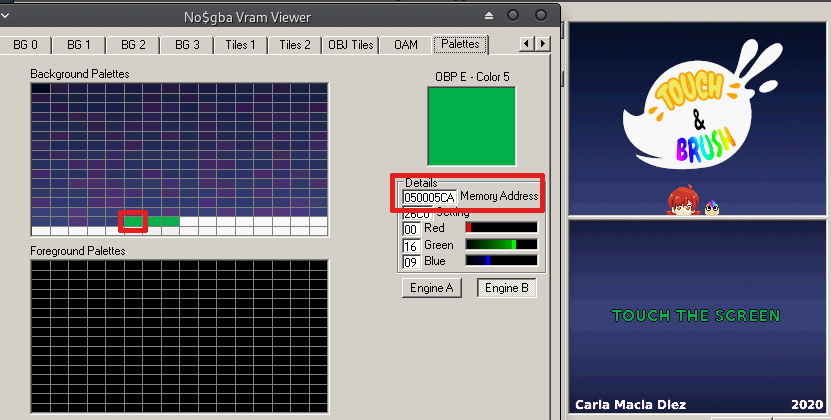
\includegraphics[width=0.7\textwidth]{archivos/palette_fade.png}
  \caption{Posición en memoria del color específico}
  \label{fig:palette_fade}
\end{figure}

 \vspace{0.5cm}

Esta posición de memoria la guardé en mi código y mi idea era, en la función update() de Menu, que iba a ser llamada una vez por ciclo, cambiar dicho color. Pero ahora bien ¿cómo podía cambiar dicho color de manera que crease un gradiente y no fuese brusco?

 \vspace{0.5cm}

Para ello, busqué información acerca de algoritmos de degradados de colores RGB, y encontré que lo que hacían era usar las componentes del color roja, azul y verde y las hacian aumentar o decrementar para conseguir convertirlos en un valor del espectro HVS. En concreto, seguían los valores de la siguiente figura:

 \vspace{0.5cm}

\begin{figure}[htbp]
\centering
  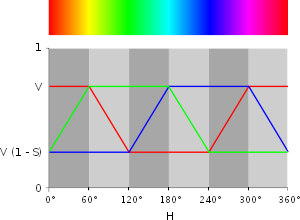
\includegraphics[width=0.7\textwidth]{archivos/rgbtohsv.png}
  \caption{Valores RGB asignados al espectro HSV}
  \label{fig:rgbtohsv}
\end{figure}

 \vspace{0.5cm}

Aprendido esto creé unas variables de tipo entero r, g y b en mi clase Graphics y ceré también una función llamada fadeTitleText() que implementa el cámbio de dichos valores. Cabe destacar que el código original de esta implementación no es propio mío, sino se encuentra publicado en la web Codepen, y es el siguiente:

 \vspace{0.5cm}

No obstante aún faltaba una cuestión, cómo transformamos estos tres valores en algo que podamos copiar en la memoria de paletas de la NDS. Para ello, libnds nos lo pone fácil, pues posee una macro llamada RGB15, que convierte los valores r g y b de 5 bits a un conjunto de 15 bits. Cabe destacar, que como estamos trabajando con componentes de 5 bits, el valor máximo de cada componente es 31, y no 255 como en el algoritmo original.

 \vspace{0.5cm}

   \begin{lstlisting}[caption={Animación del texto}, label={code:fadergb}]
void Graphics::fadeTitleText(){

    //source of the algorythm: CodePen
    //https://codepen.io/Codepixl/pen/ogWWaK/

    if(r > 0 && b == 0){
        r--;
        g++;
    }if(g > 0 && r == 0){
        g--;
        b++;
    }if(b > 0 && g == 0){
        r++;
        b--;
    }

    unsigned short color = RGB15(r,g,b);
    memcpy(TITLE_TEXT_COLOR,&color,sizeof(color));
    memcpy(TITLE_TEXT_COLOR+1,&color,sizeof(color));
    memcpy(TITLE_TEXT_COLOR+2,&color,sizeof(color));
}

\end{lstlisting}

 \vspace{0.5cm}

Al probar esto y ver que efectivamente funcionaba bien, pasé a la pantalla superior. La idea de ésta era mucho más simple, pues solo quería que se viese el fondo con el logotipo y los personajes de la historia parpadeando.

 \vspace{0.5cm}

Para realizar esto, me basé en cómo uno de nuestros referentes: Wario Ware: Touched, resuelve un problema similar. En las animaciones de las cinemáticas se utiliza mucho el recurso de separar la cara de los personajes entre el fondo y los sprites, así, las partes que siempre sean estáticas como por ejemplo la cara se mantienen ligadas a un fondo que siempre es el mismo y, las partes dinámicas como los ojos, boca, nariz, etc, se desarrollan como sprites, para que sea más fácil trabajar con ellos y ahorrar recursos.

 \vspace{0.5cm}

\begin{figure}[htbp]
\centering
  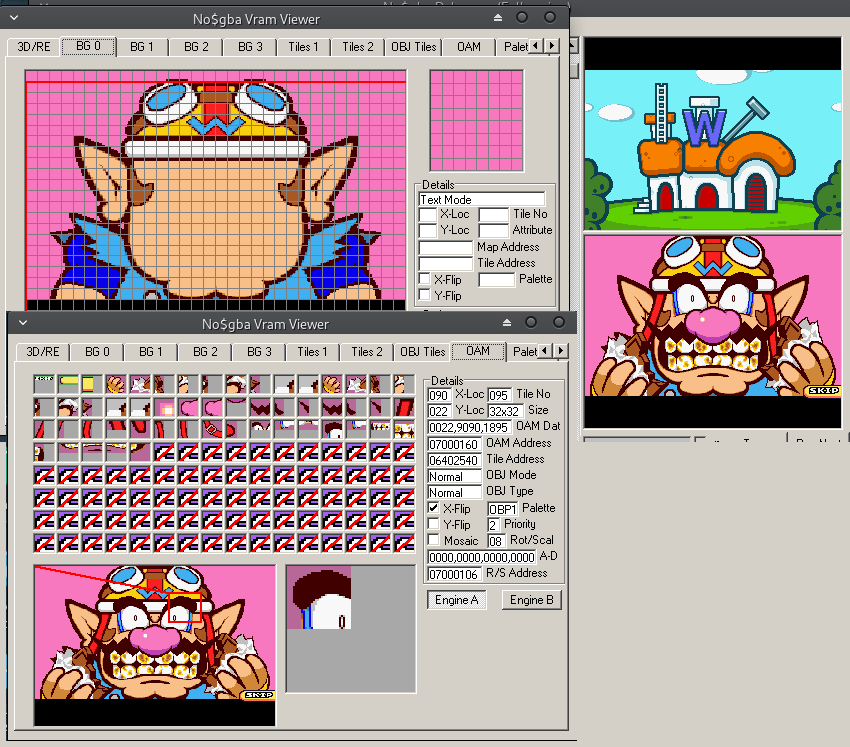
\includegraphics[width=0.7\textwidth]{archivos/wario_ware_faces.png}
  \caption{Implementación de Wario Ware: Touched de las animaciones para las cinemáticas}
  \label{fig:wario_ware_faces}
\end{figure}

 \vspace{0.5cm}

Entonces así lo hice, creé el fondo en GIMP que tenía el logotipo y las caras vacías de los protagonistas y, por separado, creé un sprite de los ojos de ambos. Incluí tanto el fondo como el sprite al menú, y mi idea para ahorrar recursos de la consola era hacer que el sprite de los ojos se escalase en el eje Y para dar la apariencia de estar pestañeando. No obstante, esto no funcionó, pues el centro de transformaciones de los sprites está situado en el centro y al escalarlo los ojos se movían de sitio. Al no poder cambiar este centro a diferencia del de los fondos, decidí hacer dicha animación por frames. Esta animación la realicé de la misma manera que las animaciones del jugador y los enemigos. 

 \vspace{0.5cm}

En la siguiente figura se muestra el resultado final de la pantalla de inicio:

 \vspace{0.5cm}

\begin{figure}[htbp]
\centering
  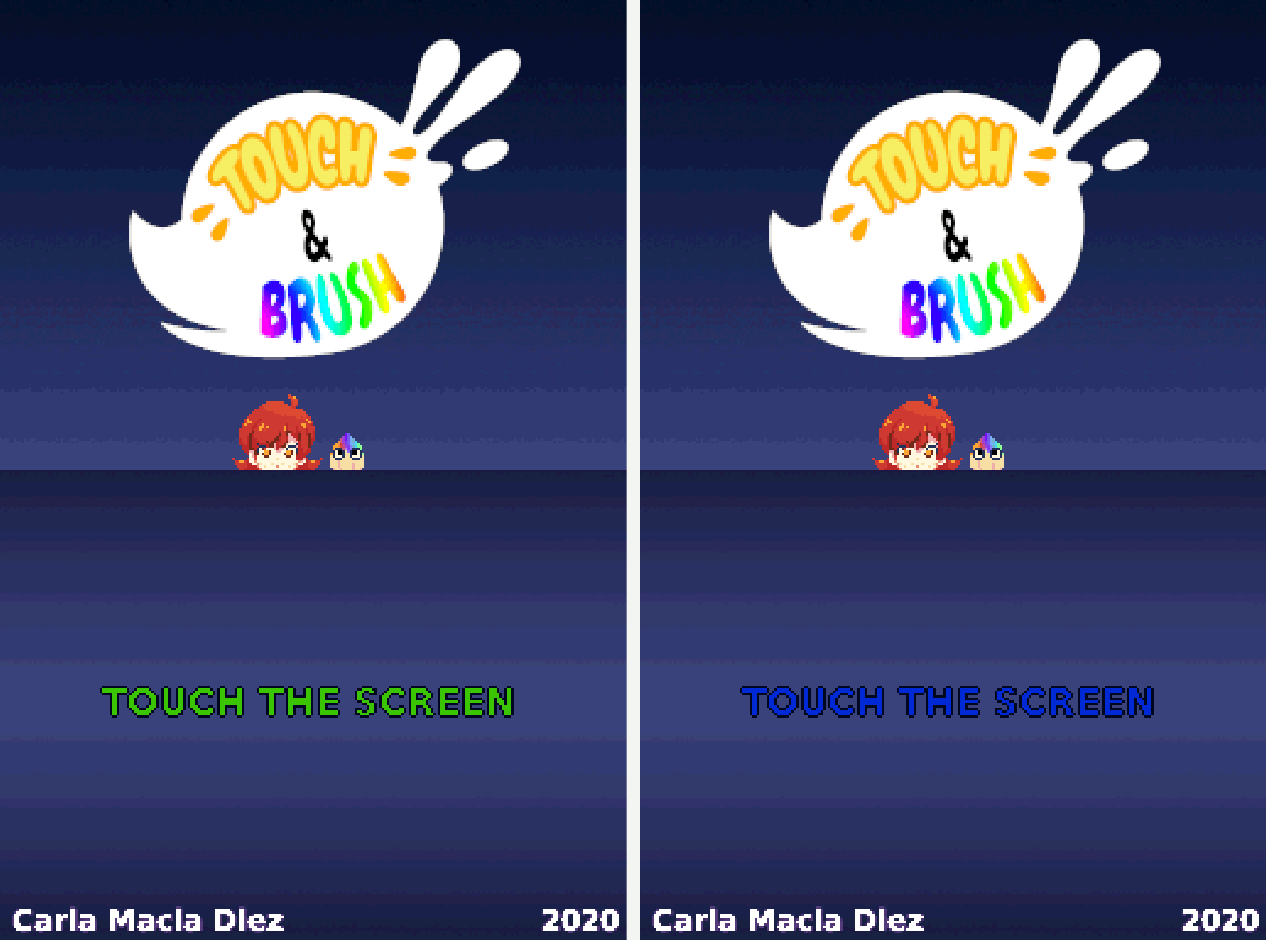
\includegraphics[width=0.7\textwidth]{archivos/menu_screen_finished.png}
  \caption{Aspecto final de la pantalla del menú principal}
  \label{fig:menu_screen_finished}
\end{figure}
\vspace{0.5cm}

Una vez terminé los aspectos visuales, pasé a centrarme en aspectos de la jugabilidad y niveles. En concreto, implementé los niveles que se diseñaron en el apartado de Diseño del juego pero para poder hacerlo tuve que hacer un pequeño cambio a los enemigos.

\vspace{0.5cm}

En cada iteración del juego, los enemigos se mueven hacia el centro de la pantalla en una unidad, pues trabajamos con coordenadas de pantalla que representan números enteros. Ahí fue donde me surgió la duda de cómo implementar las distintas velocidades, pues si aumentaba estos incrementos podrían llegar a verse saltos bruscos en los enemigos. La solución que yo pensé para esto fue hacer que tanto el incremento de los enemigos como su posición en la lógica del juego fuesen variables que representen números decimales. Sin embargo, a la hora de asignar estos valores x e y a los sprites en cada iteración los convertiremos a un entero. Esto se puede ver mejor en un ejemplo.

\vspace{0.5cm}

Imaginemos un enemigo cuya velocidad es 0.5 en el eje X y se encuentra en la coordenada 0 en ese eje. En la primera iteración, su posición pasará a ser 0.5 en ese eje, sin embargo, a la hora de asignar la posición al sprite haremos un truncamiento a ese valor decimal y pasará a ser 0. En la siguiente iteración, al sumar nuevamente el incremento, esta vez la posición decimal será 1, con lo que el sprite sí avanzaría de posición.

\vspace{0.5cm}

Esta solución personalmente me parece efectiva y simple, pues conseguimos resolver el problema, establecer velocidades de forma más sencilla y no cambiar drásticamente la lógica de los enemigos ni añadirles más variables.

\vspace{0.5cm}

Por otro lado, lo último que realicé durante esta iteración fué un cambio en el diseño de estos niveles y donde aparecían los enemigos. La idea de establecer las posiciones desde las que salían los enemigos en seis puntos en la pantalla es una buena idea para un juego como Magic Cat Academy, donde la pantalla de juego es amplia y los enemigos pueden verse sin problema.

\vspace{0.5cm}

Sin embargo, en nuestro caso tenemos una pantalla bastante reducida y los enemigos que salen por la parte superior tienen la desventaja de que el patrón que poseen se llega a ver casi cuando estos están alcanzando al jugador. Esto podría ser un punto que jugase a nuestra contra en la experiencia de usuario, pues si le mata un enemigo de estos podría sentir que no ha sido justo ya que él no ha podido llegar a ver el patrón a tiempo.

\vspace{0.5cm}

Por esto, decidí cambiar dichas posiciones iniciales y reducirlas a 4 posibles. El jugado ahora estará colocado en el centro superior de la pantalla y, como antes, saldrán enemigos de los lados y de las esquinas inferiores.

\vspace{0.5cm}


\begin{figure}[htbp]
\centering
  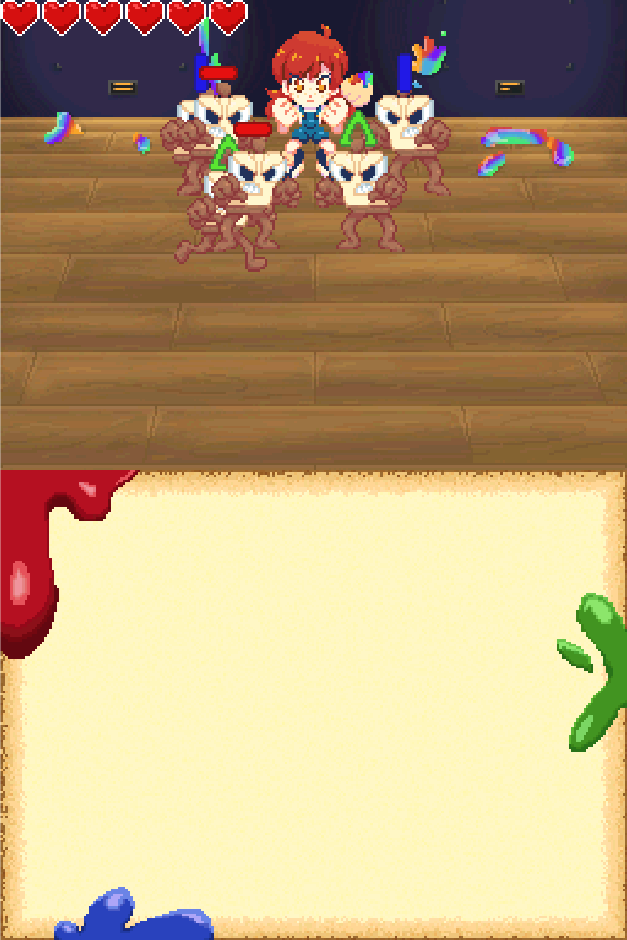
\includegraphics[width=0.4\textwidth]{archivos/finale.png}
  \caption{Posiciones finales de los enemigos.}
  \label{fig:finale}
\end{figure}

\vspace{0.5cm}

Dediqué finalmente tiempo a probar muchas veces el juego, tanto yo como amigos y familiares, y mejoraré su calidad visual incluyendo sprites de ataque y recibir daño a la protagonista. También, cambié los sprites de la vida, ya que al ser tan apagados casi no se apreciaban. 

\vspace{0.5cm}

Por otro lado, arreglé una serie de fallos, en concreto que cuando conseguías pasarte los niveles del juego y volvías al menú principal se quedaba el fondo del lienzo dibujado en la pantalla inferior. Esto es por el propio flujo del programa, ya que una vez detectamos que el usuario ha dejado de tocar la pantalla táctil, primero matamos a los enemigos y, si se considera que se ha completado el nivel, cargamos en memoria los fondos del menú principal. Sin embargo, después de eso también se llamaba al método de volver a dibujar la pantalla inferior para borrar el patrón que había dibujado el usuario. Esto estaba sobreescribiendo el fondo previamente cargado en memoria, por eso se visualizaba el del lienzo. Arreglé este fallo simplemente teniendo en cuenta que el número de enemigos a matar no fuese 0 (que significaría que ya se ha completado el nivel) para redibujar la pantalla inferior.

\vspace{0.5cm}

Por último, para mejorar la calidad del producto final y en cierto modo celebrar que el juego ya estaba completo, realicé una ilustración para la portada del videojuego.

\vspace{0.5cm}

\begin{figure}[htbp]
\centering
  \includegraphics[width=0.6\textwidth]{archivos/Touch_&_Brush_Cover_montaje.png}
  \caption{Portada de Touch \& Brush.}
  \label{fig:cover}
\end{figure}

